%%
\documentclass[english, 12pt, a4paper, elec, utf8, a-1b, online]{aaltothesis}

\usepackage{graphicx}
\usepackage{amsfonts,amssymb,amsbsy,amsmath}
\usepackage{biblatex}
\usepackage[vlined, ruled, linesnumbered, commentsnumbered]{algorithm2e}
\usepackage{multirow}

\usepackage{calc} % To reset the counter in the document after title page
\usepackage{bbm}
\usepackage{amsfonts,amssymb,amsbsy,amsmath}
\usepackage{mathtools}
\usepackage[inline]{enumitem}
\usepackage{bm}
\usepackage[vlined, ruled, linesnumbered, commentsnumbered]{algorithm2e}
\usepackage{caption}
\usepackage{subcaption}
\usepackage{gensymb}
\usepackage{outlines}



\addbibresource{references.bib}

\newcommand{\tr}[1]{\texttt{Tr}\left\{ #1 \right\}}
\newcommand{\Pest}{P_{t+1|t}^{(k)}}
\newcommand{\etal}{\textit{et al}.~}
\newcommand{\Epolicy}[1]{\mathrm{E}_\pi \left[ #1 \right]}
\newcommand{\Ss}{\mathcal{S}}
\newcommand{\As}{\mathcal{A}}
\newcommand{\Rs}{\mathcal{R}}
\newcommand{\Ps}{\mathcal{P}}
\newcommand{\Os}{\mathcal{O}}
\newcommand{\Ops}{\Omega}
\newcommand{\argmax}{\text{argmax}}
\newcommand{\egreedy}{$\epsilon$-greedy~}
\newcommand{\E}[1]{\mathrm{E}\left[ #1 \right]}
\newcommand{\inv}[1]{#1^{-1}}
\renewcommand{\Pr}[1]{\text{Pr}\left\{ #1 \right\}}

\newcommand{\xprior}{\hat{\vec{x}}_{k|k-1}}
\newcommand{\xpost}{\hat{\vec{x}}_{k|k}}
\newcommand{\xlast}{\hat{\vec{x}}_{k-1|k-1}}

\newcommand{\priorecov}{\boldsymbol{\Sigma}_{k|k-1}}
\newcommand{\postecov}{\boldsymbol{\Sigma}_{k|k}}
\newcommand{\lastecov}{\boldsymbol{\Sigma}_{k-1|k-1}}
\newcommand{\ecov}{\boldsymbol{\Sigma}_k}

\newcommand{\prefitinnov}{\Tilde{\bm{y}}_k}
\newcommand{\postfitinnov}{\Tilde{\bm{y}}_{k|k}}

\renewcommand{\vec}[1]{\mathbf{#1}}
\renewcommand{\Vec}[1]{\boldsymbol{#1}}


\newcommand{\x}{\bm{x}_k}
\newcommand{\xnext}{\bm{x}_{k+1}}
\newcommand{\xest}{\hat{\vec{x}}_k}

\newcommand{\z}{\bm{z}_k}
\newcommand{\znext}{\bm{z}_{k+1}}

\newcommand{\stmodel}{\vec{F}_k}
\newcommand{\cimodel}{\vec{B}_k}
\newcommand{\cinput}{\vec{u}_k}
\newcommand{\pnoise}{\vec{w}_k}
\newcommand{\omodel}{\vec{H}_k}

\newcommand{\onoise}{\vec{v}_k}
\newcommand{\ocov}{\vec{R}_k}
\newcommand{\pcov}{\vec{Q}_k}
\newcommand{\innocov}{\vec{S}_k}

\newcommand{\eye}{\vec{I}}
\newcommand{\gain}{\vec{K}_k}

\newcommand{\normal}[2]{\mathcal{N}\left(#1, #2 \right)}
\newcommand{\xnormal}[3]{\mathcal{N}\left(#1; #2, #3\right)}

\newcommand{\Pd}{P_\text{D}}
\newcommand{\Pfa}{P_\text{FA}}
\newcommand{\SNR}{\text{SNR}}
\newcommand{\SN}{\text{SN}_0}

\renewcommand{\exp}[1]{\text{exp}\left( #1 \right)}
\newcommand{\transpose}[1]{#1^\text{T}}
\newcommand{\rotmat}{\mathbf{T}}

\newcommand{\tmax}{t_\text{max}}
\newcommand{\tmin}{t_\text{min}}
\newcommand{\nmax}{n_\text{max}}
\newcommand{\muca}{\mu_{\text{CA}}}
\newcommand{\mucv}{\mu_{\text{CV}}}

\newcommand{\stprobs}{\vec{P}}

\newcommand{\lastmxprobs}{\mu^{j|i}_{k-1|k-1}}
\newcommand{\mxnorm}{ \Bar{c}_i }
\newcommand{\xmxinit}{\hat{\vec{x}}^{0i}_{k-1|k-1}}
\newcommand{\ecovmxinit}{\bm{\Sigma}^{0i}_{k-1|k-1}}
\newcommand{\modexlast}{\hat{\vec{x}}^{j}_{k-1|k-1}}
\newcommand{\modexprior}{\hat{\vec{x}}^{i}_{k|k-1}}
\newcommand{\modecovlast}{\bm{\Sigma}^j_{k-1|k-1}}
\newcommand{\modecovprior}{\bm{\Sigma}^i_{k|k-1}}
\newcommand{\modeinnovcov}{\mathbf{S}^i_{k}}
\newcommand{\modemxcovlast}{\Tilde{\bm{\Sigma}}^{ij}_{k-1|k-1}}
\newcommand{\modexpost}{\hat{\vec{x}}^{i}_{k|k}}
\newcommand{\modecovpost}{\bm{\Sigma}^i_{k|k}}

\newcommand{\priorecovth}{\bm{\Sigma}_{\text{th}}}

\newcommand{\deltalim}{\Delta_\text{lim}}


\DeclarePairedDelimiter\ceil{\lceil}{\rceil}
\DeclarePairedDelimiter\floor{\lfloor}{\rfloor}


\degreeprogram{Computer, Communication and Information Sciences}
\major{Signal, Speech and Language Processing}
\code{ELEC3031}
\univdegree{MSc}
\thesisauthor{Petteri Pulkkinen}
\thesistitle{Reinforcement Learning Based Radar Resource Management}
\place{Espoo}
\date{1.6.2020}
\supervisor{Prof.\ Visa Koivunen}
\advisor{Dr Tuomas Aittomäki}


%% \uselogo{aaltoRed|aaltoBlue|aaltoYellow|aaltoGray|aaltoGrayScale}{?|!|''}
\uselogo{aaltoBlue}{''}

\keywords{reinforcement learning\spc radar}

\thesisabstract{
Your abstract in English. Keep the abstract short. The abstract explains your 
research topic, the methods you have used, and the results you obtained. In the 
PDF/A format of this thesis, in addition to the abstract page, the abstract text is 
written into the pdf file's metadata. Write here the text that goes into the 
metadata. The metadata cannot contain special characters, linebreak or paragraph 
break characters, so these must not be used here. If your abstract does not contain 
special characters and it does not require paragraphs, you may take advantage of 
the abstracttext macro (see the comment below). Otherwise, the metadata abstract 
text must be identical to the text on the abstract page.
}

\copyrighttext{Copyright \noexpand\copyright\ \number\year\ \ThesisAuthor}
{Copyright \copyright{} \number\year{} \ThesisAuthor}


%% All that is printed on paper starts here
%%
\begin{document}

%% Create the coverpage
%%
\makecoverpage

%% Typeset the copyright text.
%% If you wish, you may leave out the copyright text from the human-readable
%% page of the pdf file. This may seem like a attractive idea for the printed
%% document especially if "Copyright (c) yyyy Eddie Engineer" is the only text
%% on the page. However, the recommendation is to print this copyright text.
%%
\makecopyrightpage

%% Note that when writting your thesis in English, place the English abstract
%% first followed by the possible Finnish or Swedish abstract.

%% Abstract text
%% All the details (name, title, etc.) on the abstract page appear as specified
%% above.
%%
\begin{abstractpage}[english]
  Your abstract in English. Keep the abstract short. The abstract explains your
  research topic, the methods you have used, and the results you obtained.  
  
  The abstract text of this thesis is written on the readable abstract page as
  well as into the pdf file's metadata via the $\backslash$thesisabstract macro
  (see above). Write here the text that goes onto the readable abstract page.
  You can have special characters, linebreaks, and paragraphs here. Otherwise,
  this abstract text must be identical to the metadata abstract text.
  
  If your abstract does not contain special characters and it does not require
  paragraphs, you may take advantage of the abstracttext macro (see the comment
  below).
\end{abstractpage}

\newpage
%%
%% Abstract in Finnish.  Delete if you don't need it. 
%%
\thesistitle{Vahvistusoppiminen maalinseuranta menetelmissä}
\supervisor{Prof.\ Visa Koivunen}
\advisor{TkT Tuomas Aittomäki}
\degreeprogram{Tietojenkäsittely, Tietotekniikka ja Informaatioteknologia}
%\department{Elektroniikan ja nanotekniikan laitos}
\major{Signaalin-, Puheen- ja Kielenkäsittely}
\keywords{Vahvistusoppiminen \spc tutka}
%% Abstract text
\begin{abstractpage}[finnish]
  Tiivistelmässä on lyhyt selvitys
  kirjoituksen tärkeimmästä sisällöstä: mitä ja miten on tutkittu,
  sekä mitä tuloksia on saatu. 
\end{abstractpage}

%% Force new page so that the Swedish abstract starts from a new page
\newpage

%% Preface
%%
%% This section is optional. Remove it if you do not want a preface.
\mysection{Preface}

\vspace{5cm}
Otaniemi, 1.6.2020

\vspace{5mm}
{\hfill Petteri T.\ Pulkkinen \hspace{1cm}}

\newpage

%% Table of contents. 
%%
\thesistableofcontents


%% Symbols and abbreviations
\mysection{Symbols and abbreviations}

\subsection*{Symbols}

\begin{tabular}{ll}
$q$ & Quality-value \\
$\pi$ & Policy \\
$\pi^*$ & Optimal policy \\
$k$ & Time at instant $k$\\
$\ecov$ & Predicted error covariance matrix \\
$\stmodel$ & State-transition model \\
$\pnoise$ & Process noise \\
$\omodel$ & Observation model \\
$\onoise$ & Observation noise \\
$\cinput$ & Control input \\
$\cimodel$ & Control input model \\
$\pcov$ & Process noise covariance matrix \\
$\ocov$ & Observation noise covariance matrix \\
$\stprobs$ & State-transition probabilities of a Markov chain
\end{tabular}

\subsection*{Abbreviations}

\begin{tabular}{ll}
AESA & Adaptive Electronically Scanned Arrays \\
TBM & Time budget management \\
MDP         & Markov decision process \\
POMDP      & Partially observable Markov decision process \\
RL & Reinforcement learning \\
HMM & Hidden Markov Model \\
IMM & Interacting Multiple Model \\
MSE & Mean square error \\
STS & Slow time scale \\
FTS & Fast time scale \\
JMLS & Jump Markov linear system \\
LSTM & Long short-term memory
\end{tabular}


\cleardoublepage

\section{Introduction}

A modern air surveillance radar can carry out multiple different radar functions simultaneously.
Those functions include target tracking, target classification, and search for undetected targets.
Radars that can carry out multiple different functions are generally called multifunction radars.
The key technology that has enabled multiple functions to be performed concurrently is phased-array technology such as
Adaptive Electronically Scanned Arrays (AESA).
The phased array technology enables radars to electronically steer the electromagnetic energy to the desired directions as well as receive signals from desired directions with relatively low delay.

An important problem in multifunction radars is to determine how to share the limited time budget among the different tasks.
Consequently, phased-array technology creates a great opportunity to improve air surveillance radar performance by using more efficient time budget management (TBM) algorithms.
The performance of a TBM algorithm is typically dependent on the following quantities 
\begin{enumerate*}[label=(\roman*)]
    \item the number of tracks the radar is capable to handle simultaneously,
    \item the tracking accuracy requirements, and
    \item the probability of observing undetected targets in the surveillance volume.
\end{enumerate*}
An efficient TBM algorithm is needed to maximize the benefit of using adaptive phased-array technology.

Assigning the radar time resources for multiple tasks in multifunction radars have been intensively studied by the research community.
Different names have emerged for the problem such as resource management \cite{Wintenby2006, Charlish2015a} and scheduling \cite{Esfahani2012, Byrne2015, Byrne2016, Krishnamurthy1999, Krishnamurthy2001}.
In general, resource management is intended to denote controlling any of the radar resources such as energy budget, time budget, phase shifting budget, and processing budget \cite{Ding2008}.
Moreover, the scheduling can be interpreted as to be a low-level scheduling algorithm \cite{Wintenby2006}.
In this thesis, the term "time budget management" is used, because it does not assign any expectations on how the actual objective is achieved.

Reinforcement learning (RL) has gained a great interest in the research community during recent years.
Specifically, the deep learning techniques have enabled applying RL to application domains that were before considered too difficult.
A survey by Luong \etal reveals that many different tasks can be approached with deep reinforcement learning techniques in communications and networking applications \cite{Luong2018}.
Other research areas that have shown interest in RL are for example robotics \cite{Kober2013} and smart grids \cite{Zhang2018}.
On the other hand, 
RL for radar applications has not been researched as extensively.
However, Hayking in \cite{Haykin2006} assumed that RL based approaches would be a significant direction for cognitive radar technology.
Current research papers in RL for radars considered 
jamming strategies \cite{Qiang2017, Wang2019, Wang2019a, Zhang2019},
anti-jamming strategies \cite{Kang2018, Ak2019}, 
bandwidth allocation in environments with interfering communications system \cite{Selvi2018, Kozy2019},
selecting transmit frequency to improve detection performance in environments with clutter \cite{Wabeke2010}, 
information-theoretic time budget management for multitarget tracking \cite{Kreucher2005, Xu2010},
a low-level scheduling algorithm for multichannel multifunction radars \cite{Shaghaghi2018},
selecting number of angle cells to be included into beam pattern in colocated MIMO radar \cite{Wang2018}, 
and sequential operation mode selection to improve detection performance for moving radar platform \cite{Smits2008}.

In this thesis, a reinforcement learning approach is proposed to address the TBM problem.
Moreover, a reinforcement learning algorithm is applied to control the revisit interval of the tracking filter, 
which defines the time when the tracking task is revisited.
The goal is to release time resources from target tracking to other radar functions when the target movement is more predictable.
A reinforcement learning approach may be able to learn directly from the experience such that the system model is not needed to optimize the employed reward function.
For example, a RL algorithm could be applied to different tracking filters with minimal modification on the actual reinforcement learning formulation.  
Moreover, RL methods can learn to utilize observation data with a non-trivial connection to the revisit interval.
It was shown in \cite{Charlish2015} that the partially observable Markov decision process (POMDP) framework can be utilized to introduce anticipation for controlling the revisit interval.
The reinforcement learning approach can include the anticipation for taking long-term consequences in account when planning the 
tracking revisit intervals.


\newpage
\section{Theoretical background}

A solid understanding in reinforcement learning and partially observable Markov decision processes is needed to solve the TBM problem using RL techniques.
In this chapter, the fundamental concepts are covered which are utilized in the reinforcement learning based TBM approach.
Especially, the concepts include fully observable and partially observable Markov decision processes, target tracking algorithms, and reinforcement learning algorithms.


\subsection{Markov chains} \label{sec:MC}

\begin{figure}[b]
    \centering
    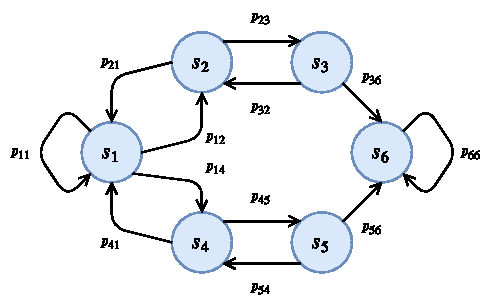
\includegraphics[width=0.8\textwidth]{figures/MarkovChain.pdf}
    \caption{
    An example of a Markov chain with six states. 
    The non-zero state transition probability from state $s_i$ to $s_j$ is written as $p_{ij}$.
    The state transition probability is zero if no arrow exists between the state pair. }
    \label{fig:mc}
\end{figure}


Consider a system which contain finite number of states that describe the operation point of the system.
The system state can sequentially transition from state to another state based on a certain stochastic model.
A Markov chain is a stochastic model which can model the sequential state transitions if the transitions are memoryless.
The memoryless transition for state $S_k$ at time instant $k$ means that   
\begin{equation} \label{eq:markov_property}
    \Pr{S_{k+1} | S_k, S_{k-1}, ..., S_1, S_0} = \Pr{S_{k+1} | S_k}.
\end{equation}
In other words, the state transition probabilities are dependent only on the current state.
The property in equation \eqref{eq:markov_property} is known as Markov property.

Next, the notation for the Markov chains is clarified.
A Markov chain has $N$ states which are represented as $s_i \in \{s_1, s_2, ..., s_N\}$.
The state transition probability from state $s_i$ to state $s_j$ is defined as $\Pr{S_k=s_j | S_{t-1}=s_i}=p_{ij}$.
Moreover, it is possible to summarize the Markov chain dynamics with a state transition matrix $\stprobs$ in which the row $i$ and the column $j$ corresponds to the probability $p_{ij}$.
An example of a Markov chain with six states is shown in Figure \ref{fig:mc}.

\subsection{Markov decision process} \label{sec:MDP}

\begin{figure}
    \centering
    \begin{subfigure}[b]{0.45\textwidth}
        \centering
        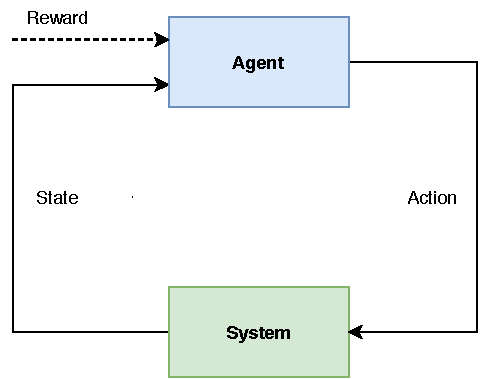
\includegraphics[width=0.9\textwidth]{figures/MDP.pdf}
        \caption{
        In an MDP, the agent takes an action that interacts with the system.
        After the action is taken, the agent receives a reward and observes the new system state.
        The reward can be dependent on the action and the state transition.
        The new system state is used to decide the next action.}
        \label{fig:mdp}
    \end{subfigure}
    \hfill
    \begin{subfigure}[b]{0.45\textwidth}
        \centering
        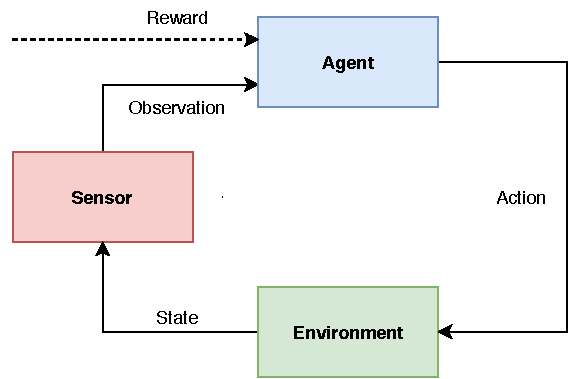
\includegraphics[width=\textwidth]{figures/POMDP.pdf}
        \caption{
        A POMDP is an extended MDP where the system state is observed through a sensor.
        The sensor can be for example a radar, and the measurements provide noisy and partial state of the system. 
        In comparison to the MDP, the reward function can be additionally dependent on the observations.
        }
        \label{fig:pomdp}
    \end{subfigure}
    \caption{Markov decision process (MDP) and partially observed Markov decision process (POMDP) visualized. }
    \label{fig:my_label}
\end{figure}

A sequential decision process is process where a decision-maker needs to sequentially make decisions that affect future decisions \cite{LaValle2006}.
If the outcomes of the decisions are not deterministic, then the decision process is considered as a stochastic decision process.
A Markov decision process (MDP) is a mathematical framework that is used to formalize the stochastic sequential decision problems \cite{Sutton2018}.
The key element of an MDP is that the system is modeled as a Markov chain.
The decision-maker in an MDP is called an agent.
The agent can choose different actions that interact with the system.
Moreover, the interaction activates a state transition of the Markov chain, and the state transition probabilities $p_{ij}$ can be dependent on the action.
After the state transition, the agent receives a reward.
The reward is dependent on which action was taken and on the state transition.
The MDP is typically described with a 4-tuple $\left( \Ss, \As, \Rs, \Ps \right)$ where $\Ss$ is the state space, $\As$ is the action space, $\Ss$ is the reward space, $\Ps$ the space that defines the transition probabilities.
The dynamics of an MDP can be summarized with a single probability distribution
\begin{equation}\label{eq:MDP_probs}
    p(s', r | s, a) = \Pr{ S_{k+1}=s', R_{k+1}=r | S_k=s, A_k=a }.
\end{equation}
which is the probability that system changes from state $s \in \Ss$ to state $s' \in \Ss$ and agent receives immediate reward $r \in \Rs$ when action $a \in \As$ is taken.
In general, the notation $X_{k}=x$ means that $x$ is the realized value for the random variable $X$ at time instant $k$.  

The objective of an agent is to collect as large rewards as possible.
A MDP problem can last for finite of infinite number of steps and the number of the steps is called horizon.  
Since an infinite horizon MDPs are considered here, the agent desires to maximize the sum of discounted future rewards.
The sum of future rewards discounted with a discount factor $\lambda$ is defined as
\begin{equation}\label{eq:discounted_sum}
    G_k = \sum_{i=0}^{\infty} \lambda^i R_{k + i + 1}
\end{equation}
where $R_{t+k+1}$ is the reward received from taking action $A_{t+k}$. 

In MDP it is assumed that the system state is fully observable.
Therefore, the agent needs to find a policy $\pi(a | s)$ which gives the probability for taking action $a \in \As$ given the state $s \in \Ss$.
The optimal policy is defined as
\begin{equation}\label{eq:mdp_optimal_policy}
    \pi^* = \arg\max_\pi\Epolicy{G_k | S_k}.
\end{equation}
which is the policy that gains the greatest expected discounted sum of rewards.
By the definitions \eqref{eq:discounted_sum} and \eqref{eq:mdp_optimal_policy}, the optimal policy would need to consider all the future actions.
Such policies are called non-myopic policies.
In comparison, a policy where the agent maximizes the immediate reward is called a myopic policy. 
Typically, the myopic policies are suboptimal for $\lambda>0$.

Since an optimal policy maximizes discounted sum of expected future rewards, a reasonable way to evaluate policy $\pi$ is to use a value function which is defined as follows
\begin{equation} \label{eq:value}
    v_\pi(s) = \Epolicy{G_k | S_k=s}.
\end{equation}
The value function gives the expectation of the discounted rewards given the initial state $s$ which quantifies the quality of the state given the policy $\pi$.
Moreover, the optimal policy $\pi^*$ has always greater or equal values for any state $s \in \Ss$ compared to any other policy $\pi$.
Similarly, another metric that can measure the quality of any action $a \in \As$ given the state $s \in \Ss$ is defined as
\begin{equation}\label{eq:action_value}
    q_\pi(s, a) = \Epolicy{G_k | S_k=s, A_k=a},
\end{equation}
and it is called an action-value function.
It is quite straightforward to prove that the value function \eqref{eq:value} can be expressed in a recursive form 
\begin{align}
    v_\pi(s) 
    &= \Epolicy{ \sum_{i=0}^{\infty} \lambda^i R_{k + i + 1} | S_k=s} \\
    &= \Epolicy{R_{k + 1} + \lambda \sum_{i=0}^{\infty} \lambda^i R_{k + i + 2} | S_k=s} \\
    &= \sum_{a \in A} \pi(a | s) \sum_{s' \in S} \sum_{r \in R} p(s', r | s, a) \left[ r + \lambda v_\pi(s') \right]\label{eq:bellman},
\end{align}
where \eqref{eq:bellman} is called Bellman equation.
The Bellman equation is the key for solving MDPs because it enables using recursion such as dynamic programming to calculate the values \eqref{eq:value} or action-values \eqref{eq:action_value}.


\subsection{Partially observable Markov decision process} \label{sec:POMDP}


A partially observable Markov decision process (POMDP) is an extension to MDP which was introduced in Section \ref{sec:MDP}. 
The difference between the POMDP and the MDP is that the Markov chain state is not fully observable \cite{Krishnamurthy2016}.
Moreover, a Markov chain that is not fully observable is called a hidden Markov model (HMM).
In real-world systems, the state of the Markov chain is usually partially observable because sensors can contain noise or the observation does not contain full information about the state.
The POMDP framework extends the MDP 4-tuple with observation space $\Os$ and observation probability space $\Ops$ such that a POMDP problem is described with a 6-tuple $(\Ss, \As, \Rs, \Ps, \Os, \Ops)$.
The observation space describes all the observations that the agent can observe.
Moreover, the observation probability $o(z|s, a) \in \Ops$ defines the probability of obtaining the observation $z \in \Os$ given the state $s \in \Ss$ and the action $a \in \As$.
Thus, the agent can affect the observation probabilities in addition to the state transition probabilities. 

Generally, a policy that is used to address a POMDP problem is dependent on the complete history of the past actions and observations. 
The history is called the information history.
The information history until time instant $k$ is written as $I_k=\{A_0, O_0, A_1, O_1, ..., A_k, O_k\}$, where $A_k \in \As$ and $O_k \in \Os$ are the action and the observation at time instant $k$, respectively.
It is possible to combine the information $I_k$ to form a belief state distribution $b(s)$ which indicates the probability of a Markov chain being on a state $s$.
Thus, the policy can be written as $\pi(a | b)$, which is the probability of choosing the action $a$ given the belief state $b$.
The belief state can be updated with an Bayesian update rule, which is written as follows
\begin{equation}\label{eq:belief_state_update}
    b_{k+1}(s) = \frac{o(z | s, a) \sum_{s'\in S} \Pr{s | s', a} b_k(s')}{\sum_{s'\in S, s'' \in S} \Pr{s'' | s', a} \Pr{z | s'', a)b_k(s')}}.
\end{equation}
An approach to solve a POMDP is to formulate the problem as a continuous state MDP where the belief state $b$ is used as a state variable instead of using the state variable $s$.

\subsection{Reinforcement learning} \label{sec:RL}

Reinforcement learning (RL) is a method for learning to act in stochastic sequential decision-making problems without a model that describes the system dynamics \cite{Sutton2018}. 
An RL problem is formulated as an MDP where the transition probabilities and reward distributions are unknown. 
Thus, defining the state space, the action space, and the rewards are an essential part of formulating a problem as a reinforcement learning problem.
The agent learns a suitable policy from received feedback. 
Basically, the feedback contains an observation that is related to the state of the system and a reward that helps the agent to evaluate consequences for its actions given the observation history. 
The policy of the RL agent can be measured with value and action-value functions similarly as shown in Section \ref{sec:MDP}.

The rewards for the RL agent are defined such that the objective is achieved by maximising the equation \eqref{eq:discounted_sum} \cite{Sutton2018}.
For example, if RL is used to teach a robot to play chess, then positive reward should be given if the robot wins and otherwise no reward is given.
Then, the value function \eqref{eq:value} indicates the probability of winning given the current game state.

The MDP and POMDP theory in Section \ref{sec:MDP} and Section \ref{sec:POMDP} considered state and action spaces with finite cardinality. 
To apply RL techniques for continuous state and action spaces, function approximators have been employed to approximate the value or action-value functions \cite{Sutton2018}. 
Especially, deep neural networks have been widely adopted to solve RL problems with continuous state and action spaces in different application domains \cite{Zhang2018, Luong2018}.
However, the training required to train deep RL agent can get quite intensive \cite{Irpan2018}.
For RL problems that involve neural networks, the models are usually trained with simulations and then fine-tuned in the real environment.

\subsubsection{Exploration and exploitation}

Exploration and exploitation is an essential concept in RL which allows the RL agent to improve the policy by simple trial-and-error method.
Initially, the agent starts with no knowledge about the system dynamics meaning that the initial policy is random.
Therefore, the agent needs to utilize a policy for probing different actions that have unknown consequences.
The probing is used to gain more knowledge about the dynamics, and the increased knowledge can be utilized to improve the policy.
The actions that are taken to gain more knowledge are called exploration actions.
Otherwise, the agent chooses the action that is believed to be the best action which is called exploitation.
The dilemma of finding the balance between exploration and exploitation is called exploitation-exploitation trade-off.

Widely used policy for balancing the exploration-exploitation trade-off is called \egreedy policy \cite{Sutton2018}.
With \egreedy policy, the agent chooses random action with probability $\epsilon$.
When not choosing the action randomly, the action with highest action-value is chosen.
Therefore, the policy can be written as follows
\begin{equation}
    a =
    \left\{
        \begin{array}{ll}
            \arg\max_{a' \in A} q_\pi(s, a') & \text{with probability $1-\epsilon$}\\
            \text{random action} & \text{with probability $\epsilon$}.
        \end{array}
    \right.
\end{equation}
where $a$ is the chosen action and $0 < \epsilon \ll 1$.

With fixed exploration parameter $\epsilon$, the optimality can not be achieved since random actions will be always taken.
One solution is to gradually decay the parameter $\epsilon$, but specifying the decay rate can be tedious without causing a significant change in the convergence speed.
Most of the other exploration and exploitation policies that have been proposed in the literature are not suitable for solving general RL problems \cite{Slivkins2019}.
Instead, they are suitable for a particular RL problem called stochastic multi-armed bandits which are MDPs with one state.

\subsubsection{Q-learning}

Probably the simplest, yet effective reinforcement learning algorithm is Q-learning algorithm.
The Q-learning algorithm is a temporal difference learning algorithm which utilizes the recursion in Bellman equation \eqref{eq:bellman}.
The Bellman equation is solved iteratively by initializing the Q-values with arbitrary values and updating them using Monte Carlo simulations.

\begin{algorithm}[H]
    \SetAlgoLined
    Initialize $Q(s, a) \forall s \in \Ss, a \in \As$\;
    \While{Q not converged}{
    choose $a$ using policy $\pi$ ($\argmax_a Q(s, a)$ and $\epsilon$-greedy)\;
    $r, s' \leftarrow$ take action $a$\;
    $Q(s, a) \leftarrow Q(s, a) + \alpha (r + \lambda \max_a Q(s', a) - Q(s, a))$\; 
}
\caption{Q-learning algorithm \cite{Sutton2018}}
\end{algorithm}

\subsubsection{SARSA}

\subsection{Target tracking algorithms} \label{sec:Tracking}

The target kinematic state can be described as a continuous-valued stochastic process that evolves based on the target dynamics. 
Radar is used to observe the target state, but the observations contain noise and only partial information, such as position and radial velocity, of the state is obtained. 
Therefore, a target tracking algorithm is used to estimate the target state from observation history. 
Typically, a mathematical model is utilized to attenuate noise from the measurements and estimate the present and predict future states.
The most known models combine a motion model and a measurement model, which are known as state-space models \cite{RongLi2003}. 
The motion model describes how the kinematic state evolves through time.
In discrete-time, the motion model is expressed in the form of
\begin{equation}\label{eq:spm_motion}
\xnext  = f(\x, \cinput) + \pnoise,
\end{equation}
where $\pnoise$ is a noise that describes uncertainty in the model.
The measurement model describes the relationship between the target state and the observations. 
Similar to the motion model, the discrete-time measurement model is written as follows,
\begin{equation}\label{eq:spm_obs}
\z = h(\x) + \onoise,
\end{equation}
where $\onoise$ is the measurement noise.

The form of the motion model can be approximated from physics, but especially the control-input $u_k$ and the statistics of $v_k$ are unknown for the observer.
Therefore, different kinds of motion models have been developed to mimic the true target motion with certain accuracy \cite{RongLi2003}. In the higher level, the models can be divided into non-maneuvering and maneuvering models. Non-maneuvering motion means that the target velocity and elevation remains approximately constant. Otherwise, the target motion is considered to be maneuvering.

\subsubsection{Kalman filtering}

\begin{figure}[b]
    \centering
    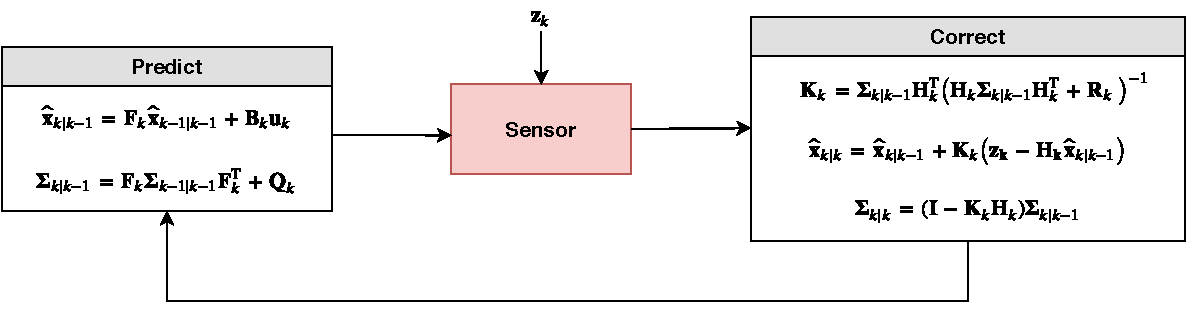
\includegraphics[width=\textwidth]{figures/KF.pdf}
    \caption{The Kalman filtering phases.
    First, the predictions of the state $\xprior$ and the error covariance $\priorecov$ are calculated.
    The predictions can be used to control the sensor, that affect observation probability covariance matrix $\ocov$ of the observation $\z$.
    After $\z$ has been observed, the predictions can be corrected by utilizing the Kalman gain $\gain$.
    }
    \label{fig:KF}
\end{figure}

Kalman filtering is an optimal state estimation approach in case when the system can be described as a linear state-space system with additive Gaussian noise \cite{Krishnamurthy2016}.
The discrete-time linear state-space model is expressed using linear combinations as follows 
\begin{align}
    \xnext &= \stmodel \x + \cimodel \cinput + \pnoise \label{eq:lsp_state} \\
    \z &= \omodel \x + \onoise \label{eq:lsp_obs}
\end{align}
where $\stmodel$ is state transition matrix, $\cimodel$ is control-input matrix, $ \omodel $ is observation matrix. 
The noise statistics are described with zero mean Gaussian distributions $\pnoise \sim \normal{0}{\pcov}$ and $\onoise \sim \normal{0}{\ocov}$, where $\pcov$ is the process noise covariance matrix and $\ocov$ is the measurement noise covariance matrix.

The Kalman filtering can be divided into two phases as shown in the Figure \ref{fig:KF}.
In the first phase, the next state is predicted from the last estimate using the equation \eqref{eq:lsp_state}.
In addition, the error covariance matrix $\ecov$, that estimates the accuracy on the estimates $\xest$, is updated based on the process noise and on the previous estimated posterior error covariance matrix.
Therefore, the predict phase can be summarized with two equations as follows,
\begin{subequations}
\label{eq:kf_predict}
\begin{align}
    \xprior &= \stmodel \xlast + \cimodel \cinput \label{eq:kf_pred_x} \\ 
    \priorecov &= \stmodel \lastecov \stmodel^T + \pcov \label{eq:kf_prior_error_cov},
\end{align}
\end{subequations}
where $\priorecov$ is the predicted prior error covariance matrix.

In the second phase, a measurement is obtained and the estimates can be updated. 
In other words, the predictions \eqref{eq:kf_pred_x} and \eqref{eq:kf_prior_error_cov} are corrected based on the obtained measurement and Kalman gain.
The update phase starts by calculating a residual between the observation $z$ and the predicted observation.
The residual is called pre-fit innovation and it is utilized to correct the prior estimate $\xprior$.
A Kalman gain defines how much the pre-fit innovation is weighted to calculate the posterior estimate $\xpost$.
The Kalman gain is found by minimizing mean squre error (MSE) between $\x$ and $\xpost$.
As a result, following update equations are obtained
\begin{subequations}
\label{eq:kf_update}
\begin{align}
    \prefitinnov &= \z - \omodel \xprior \label{eq:kf_prefit_innov}\\ 
    \innocov &= \omodel \priorecov \omodel^T + \ocov \label{eq:kf_innov_cov}\\ 
    \gain &= \priorecov \omodel^T \inv{\innocov} \label{eq:kf_gain}\\ 
    \xpost &= \xprior + \gain \prefitinnov \label{eq:kf_update_x}\\ 
    \postecov &= \left( \eye - \gain \omodel \right) \priorecov  \label{eq:kf_post_error_cov}\\
    \postfitinnov &= \z - \omodel \xpost \label{eq:kf_postfit_innov}
\end{align}
\end{subequations}
where $S_k$ is the covariance on the pre-fit innovation $\prefitinnov$. 
Even if the notation in equations \eqref{eq:kf_predict} and \eqref{eq:kf_update} suggests to use prior or posterior estimates on the previous time step, multiple predictions can be made sequentially or multiple updates can be made at each time interval.



\subsubsection{Interacting Multiple Model estimator}
\label{sec:IMM}

\begin{figure}[b]
    \centering
    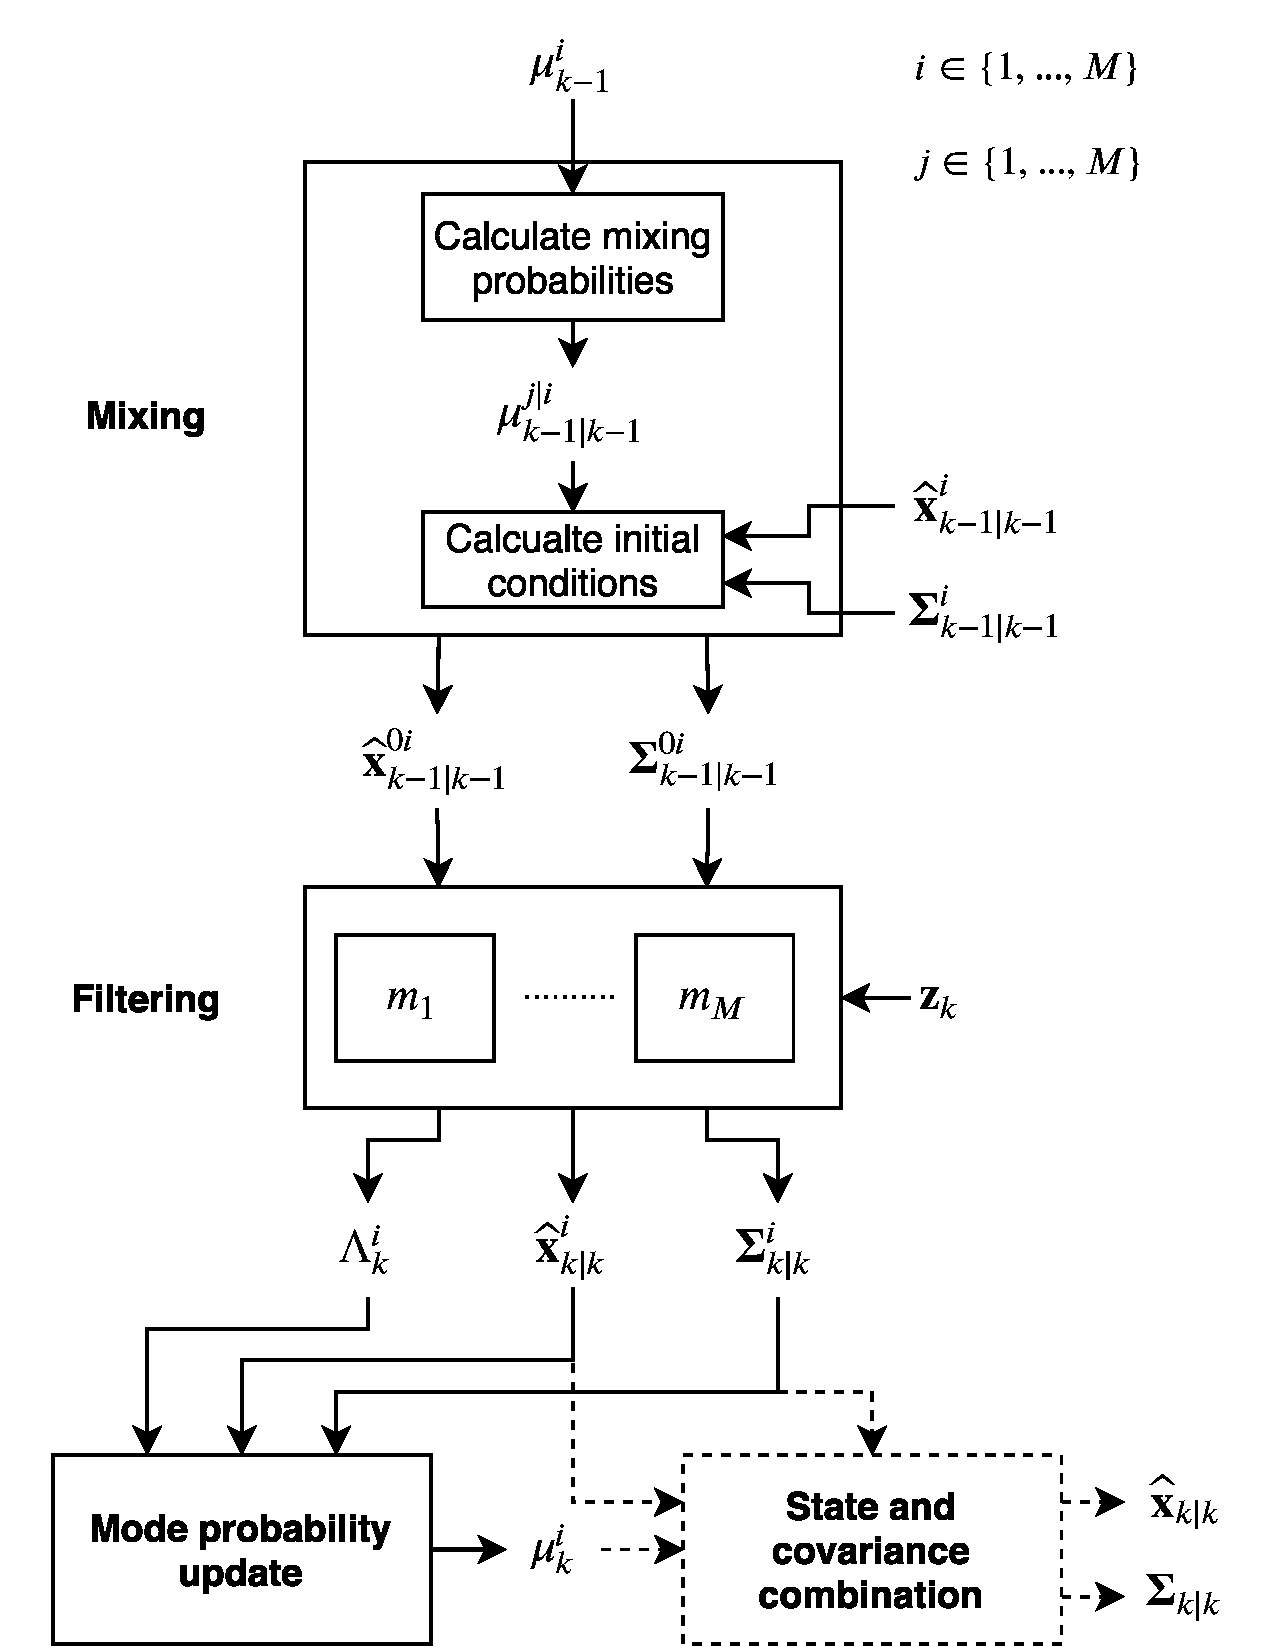
\includegraphics[width=0.7\textwidth]{figures/IMM_figure.pdf}
    \caption{
    The four steps in IMM estimation. 
    The figure is reprinted from \cite{BarShalom2001}.}
    \label{fig:IMM}
\end{figure}

In a realistic scenario, the target motion could obey different modes, and the changes between the modes are controlled by an external agent, for example by a human.
Such systems are called hybrid systems, which are characterized by a continuous-time stochastic process, such as \eqref{eq:spm_motion}, that describes the motion model for each mode and by a discrete-time stochastic process that describes the evolution of the modes \cite{Mazor1998}.
To track the state of a hybrid system effectively, an approach utilizing multiple motion models has emerged \cite{BarShalom2001}.
Moreover, the approach assumes that the target motion could be modeled approximately by a finite number of models.
The underlying mode is identified by a mode matched filter which calculates the probability of each mode given the past observations.
For an optimal approach, the number of mode matched filters would grow exponentially in the function of time, even if the modes are switched based on an HMM \cite{BarShalom2001}.
An Interacting Multiple Model (IMM) estimator is a specific suboptimal hybrid filter that achieves great trade-off between the performance and the computational complexity \cite{Mazor1998}.

An IMM estimator assumes that the target motion at each time instant can be expressed by one of the models in the finite set $\mathcal{M} = \{ m_i \}_{i=1}^M$, where $M$ is the number of the models.
The switches between the modes is described by an HMM, and the state transition probabilities of the HMM are assumed to be known.
However, in practical scenarios, the modes and the transition probabilities are considered as design parameters \cite{Simeonova2002}.
Given $Z_k$ which is the observation sequence through time $k$, the posterior probability for model $m_i$ to be in effect at time instant $k$ is written as $\Pr{m_i | Z_k} = \mu^i_{k}$.


The IMM estimator can be summarized with four steps that are shown in Figure \ref{fig:IMM}.
The steps are mixing, filtering, mode probability update, and state and covariance combination. 
The steps are further implemented as follows. 


\begin{description}
% ---------------------------------------------------------
% Mixing
% ---------------------------------------------------------
\item[Mixing.]

The mixing starts by calculating probability $\Pr{m_j(k-1)|m_i(k), Z_{k-1}}$, which is the probability that mode $m_j$ was active at last time step if the current active mode is $m_i$ given the past observations.
The probability is called mixing probability, and the equation for calculating it is written as,
\begin{equation}
    \lastmxprobs = \frac{1}{\mxnorm} p_{ji} \mu^j_{k-1} \label{eq:imm_mx_probs}
\end{equation}
where $\mxnorm$ is a normalization term. 
The normalization term is defined as follows
\begin{equation}
    \mxnorm = \sum_j^M p_{ji} \mu^j_{k-1}. \label{eq:imm_mx_normalization}
\end{equation}
The mixing probabilities are used to calculate mixed estimates for the previous posterior state variables and error covariance matrices, which are further used in the tracking filters.
Moreover, the mixed estimates are calculated for the case where it is assumed that the current mode matches to the model $m_i$ of the tracking filter.
Therefore, the estimates are calculated as follows
\begin{subequations}
\begin{align}
    \xmxinit &= \sum_j^M \lastmxprobs \modexlast \label{eq:imm_mx_init_x}\\
    \ecovmxinit &= \sum_j^M \lastmxprobs \left[ \modecovlast + \modemxcovlast \right], \label{eq:imm_mx_init_P}
\end{align}
\end{subequations}
where $\modexlast$ and $\modecovlast$ are the last state and covariance posterior estimates of the tracking filter for mode $m_j$, respectively. 
In addition, $\ecovmxinit$ is defined as follows
\begin{equation}
    \modemxcovlast = 
    \left( \xmxinit - \modexlast  \right) 
    \transpose{\left( \xmxinit - \modexlast   \right)}.\label{eq:imm_mx_init_Ptilde}
\end{equation}

% ---------------------------------------------------------
% Filtering
% ---------------------------------------------------------
\item[Filtering.]

In the filtering phase, the likelihood of the observation given the model $m_i \in \mathcal{M}$ is calculated  $\Lambda^i_k = \Pr{\z | m_i(k), Z_{k-1}} $.
The conditioning is approximated by assuming that $\xmxinit$ and $\ecovmxinit$ can be utilized to condition the filters before propagating the filtering equations.
Therefore, the likelihood is obtained from the following relation
\begin{equation}
    \z \sim \normal{\modexprior}{\modeinnovcov},
\end{equation}
where equations \eqref{eq:kf_pred_x} and \eqref{eq:imm_mx_init_x} are used to calculate $\modexprior$, and $\modeinnovcov$ is calculated by using equations \eqref{eq:kf_prior_error_cov}, \eqref{eq:kf_innov_cov}, \eqref{eq:imm_mx_init_P}.

% ---------------------------------------------------------
% Mode probability update
% ---------------------------------------------------------
\item[Mode probability update.]

The mode probabilities $\mu^i_k$ can be updated by using the likelihoods $\Lambda_k^i$ as follows
\begin{equation}
    \mu_k^i = \frac{1}{c} \Lambda^i_k \mxnorm,
\end{equation}
where
\begin{equation}
    c = \sum_{i=1}^M \Lambda_i^k \mxnorm
\end{equation}
is a normalization constant.

% ---------------------------------------------------------
% State and covariance combination
% ---------------------------------------------------------
\item[State and covariance combination.]
Lastly, the posterior estimates $\xpost$ and $\postecov$ can be updated by combining mode probabilities and posterior estimates calculated by each filter.
Thus, the estimates are calculated as follows
\begin{subequations}
\label{eq:imm_estimate}
\begin{equation}
    \xpost = \sum_{i=1}^M \mu_k^i \modexpost
\end{equation}
\begin{equation}
    \postecov = \sum_{i=1}^M \mu_k^i 
    \left[ 
        \modecovpost + \left( \modexpost - \xpost \right) \transpose{\left( \modexpost - \xpost \right)}
    \right]
\end{equation}
\end{subequations}
Note that the equations \eqref{eq:imm_estimate} are outputs of the IMM estimator, and not needed for the other IMM estimator steps.
\end{description}


\newpage
\section{Literature review on radar time budget management} \label{sec:literature_review}

The TBM problem is essentially a scheduling problem in which different radar sensing tasks are scheduled to optimize the employed utility function.
The utility function should be developed in such a way that targeted performance levels and operational goals are achieved.
A radar task has a certain starting and ending time, which specify how long the task was executed.
Moreover, the time needed to execute the task is called the dwell time.
For the track update tasks, the time interval between the track updates is called a revisit interval.
The time instances addressed here are illustrated in Figure \ref{fig:timeline}.
The time budget of the multifunction radar is shared among multiple tasks such as tracking, searching and classification.
If multiple tasks can be executed by a functional subsystem of a radar or a complete radar set, then the scheduling problem is considered to have multiple channels \cite{Shaghaghi2018}.
However, most of the research is concentrated on single channel scheduling problems e.g. \cite{Charlish2015a, Byrne2015, Byrne2016, Esfahani2012, Wintenby2006}.

The scheduling problem can be interpreted as a decision-making problem in which the decision-maker needs to decide when to execute the radar tasks and how much time is needed to execute them \cite{Wintenby2006}.  
The decision-making problem can be interpreted as a stochastic sequential decision-making problem since the radar measurements and the target dynamic models contain noise.
Moreover, the sensing decisions affect future sensing, thus the long-term consequences need to be taken into account.
The decision-making problem can be composed in the following steps 
\begin{enumerate}
    \item Get an observation of the system state,
    \item Select an action which maximizes the cumulative reward function using the belief information,
    \item Return to step one.
\end{enumerate}
Such process can be modeled as a partially observable Markov decision process (POMDP).
The state space, the observation space, the action space, and rewards are dependent on the particular problem formulation.

Different approaches for TBM have been proposed in the literature.
On a higher level, the approaches can be divided into task-based methods and rule-based methods as shown in Figure \ref{fig:tbm_categorization}.
In task-based methods, all the tasks are enumerated and a subset of the tasks are executed at the next scheduling interval.
The tasks are selected based on the current belief state of the system. 
An optimal task-based TBM approach would select a single task at a time for a given belief state with a non-myopic policy.
The non-myopic policy is essential in multifunction radars such that the long-term rewards are maximized to prevent losing target tracks or missing target detections.
The computational complexity of an optimal task-based algorithm can become intractable with realistic assumptions. 
As a consequence, Wintenby \etal proposed in \cite{Wintenby2006} a hierarchical TBM management algorithm \cite{Wintenby2006}.
The approach divides the task-based TBM problem into a slow-time-scale and fast-time-scale scheduling problems.

In the rule-based TBM, deadlines for the tasks are calculated based on certain rules, and a low-level scheduling algorithm arranges the tasks to the timeline.
Typically, fixed or adaptive revisit intervals are used, and the remaining time budget can be used for other radar tasks  \cite{Keuk1975, Cohen1986, Gardner1988, Munu1992, vanKeuk1993, Watson1993, Daeipour1994, Shin1995, Benoudnine2006, ChengTing2007, Baek2010, Charlish2015, Mofrad2017, Masoumi-Ganjgah2017, Christiansen2018, Pilte2018}.
The adaptive revisit interval algorithms can be utilized to minimize the required time budget if the low-level scheduler can schedule the actual track updates close to the desired revisit interval.
Therefore, the rule-based algorithms are heavily dependent on the scheduling algorithm and reasonable revisit intervals.


\begin{figure}[h]
    \centering
    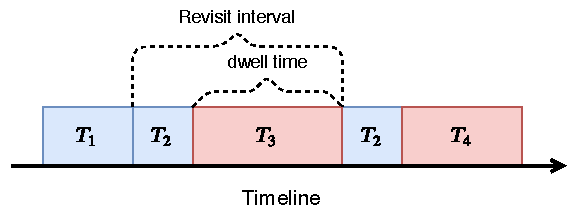
\includegraphics{figures/timeline.pdf}
    \caption{
        An example for tasks $T_i \forall i\in\{1,2,3,4\}$ that are scheduled on a radar timeline. 
        The revisit interval and dwell time is illustrated in the figure.
        The blue and red color illustrate different type of tasks such as tracking and search tasks.
        The task scheduler should generate the timeline such that cumulative reward function is maximized. 
    }
    \label{fig:timeline}
\end{figure}

\begin{figure}[h]
    \centering
    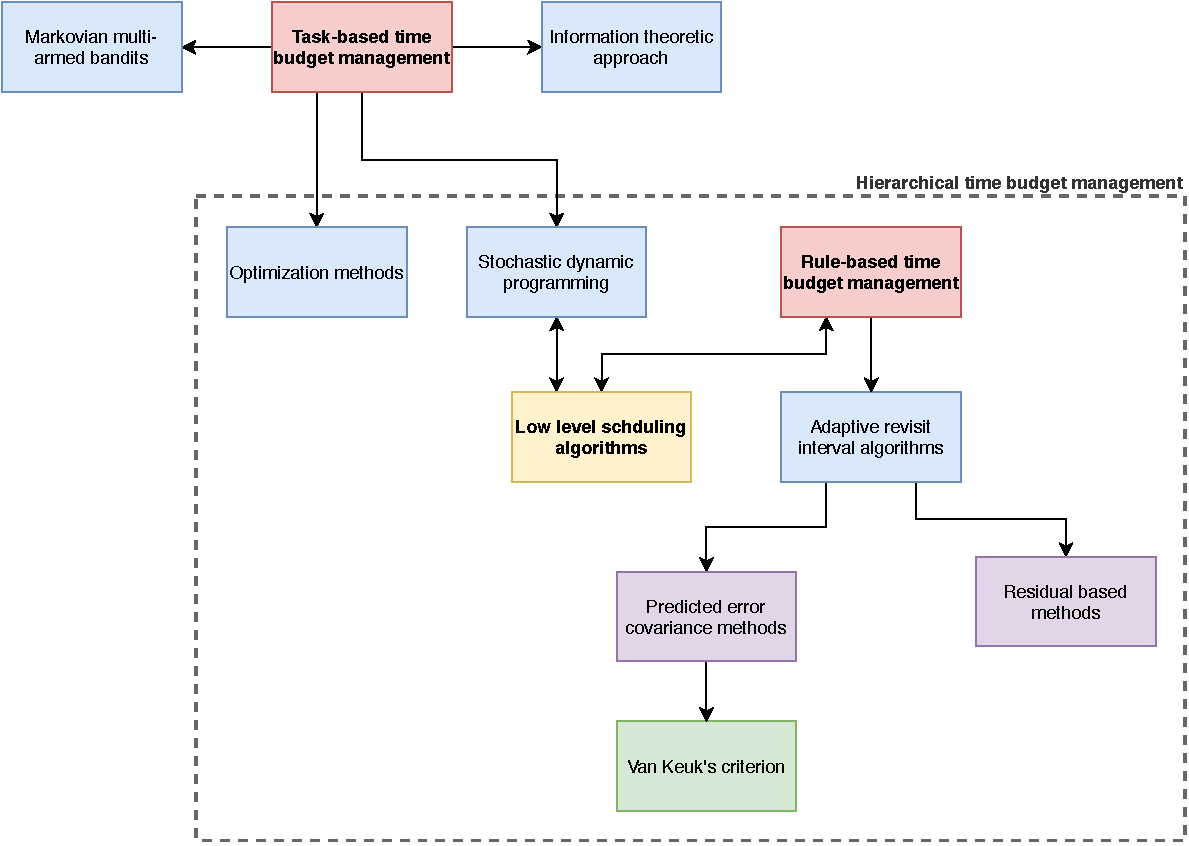
\includegraphics[width=\textwidth]{figures/TBM_algorithms.pdf}
    \caption{Categorization of the reviewed time budget management approaches.}
    \label{fig:tbm_categorization}
\end{figure}

\subsection{Task-based time budget management}

In this section, the task-based TBM covered which is the basis for an optimal TBM in multifunction radars.
Optimal task-based approaches have been proposed in \cite{Krishnamurthy1999, Krishnamurthy2001}, where multitarget tracking problem is formulated as a Markovian multi-armed bandit problem with known target dynamics.  
In addition, optimal information-theoretic TBM algorithms were introduced in \cite{Kastella1997, Kreucher2004, Kreucher2005, Xu2010}.

The computational complexity of an optimal task-based algorithm can become intractable with realistic assumptions. 
As a consequence, Wintenby \etal proposed in \cite{Wintenby2006} a hierarchical TBM management algorithm \cite{Wintenby2006}.
The approach divided the TBM problem into a slow-time-scale and fast-time-scale scheduling problems.
Later on, different task-based TBM approaches have been proposed in the literature which utilizes the two-level hierarchy \cite{Byrne2015, Byrne2016, Esfahani2012}.


\subsubsection{Multi-armed bandits for beam scheduling in multitarget tracking}

The TBM for multitarget tracking can modeled as a POMDP \cite{Krishnamurthy1999, Krishnamurthy2001, Scala2006}.
The state space of the POMDP grows exponentially in number of targets, since each target has individual dynamic states.
The large state space of the POMDP problem can be relaxed by assuming Markovian multi-armed bandit formulation, in which each target trajectory is modeled as a HMM \cite{Krishnamurthy1999, Krishnamurthy2001}.
In addition, in the multi-armed bandit formulation, the Markov state of the HMM evolves only if it has been observed.
Such assumption is inappropriate since the targets can move even if they are not observed.
The restless multi-armed formulation enables each HMM state to evolve concurrently \cite{Scala2006}.
However, the optimal solution for the RMAB problem is NP-hard \cite{Guha2007}.
Performance of a myopic solution was investigated in \cite{Scala2006}.
The target which minimizes the sum of predicted uncertainties was chosen at each scheduling interval.
The myopic policy was claimed to be optimal in the assumed simple scenario with two targets.
However, the myopic policy is suboptimal in general setting where multiple targets could exist or when the system dynamics are more complex.

\subsubsection{Information-theoretic approach for beam scheduling} \label{sec:inf_based}

A myopic information-theoretic approach for beam direction scheduling was proposed in \cite{Kastella1997}.
The surveillance area was divided into smaller grid cells.
It is possible to calculate the probability of target existing in a given grid cell based on prior probabilities and past observations. 
Moreover, the radar can decide which cells are observed by deciding the illumination direction.
The track and search tasks are joined such that observing different grid cells must minimize the uncertainty of target existence in the radar scenario.
Transition and birth probabilities for undetected targets need to be predefined for each cell when the information-theoretic approach is used.

A tractable non-myopic information based method for multitarget search and tracking was proposed in \cite{Kreucher2004}.
It used particle filtering to obtain the posterior probabilities for the target states.
Joint multitarget probability density was used to determine the probabilities of target being in the given cell.
An approximation method was used to approximate the Bellman equation in \eqref{eq:bellman} to account the long-term consequences. 
In \cite{Kreucher2005}, the approximate method was compared to an optimal non-myopic policy which was found by using Q-learning.
Different information-theoretic measures for presenting the belief state was compared in \cite{Xu2010}.
Furthermore, a deep reinforcement learning algorithm was used to approximate the Bellman equation.

\subsubsection{Hierarchical time budget management}

\begin{figure}[h]
    \centering
    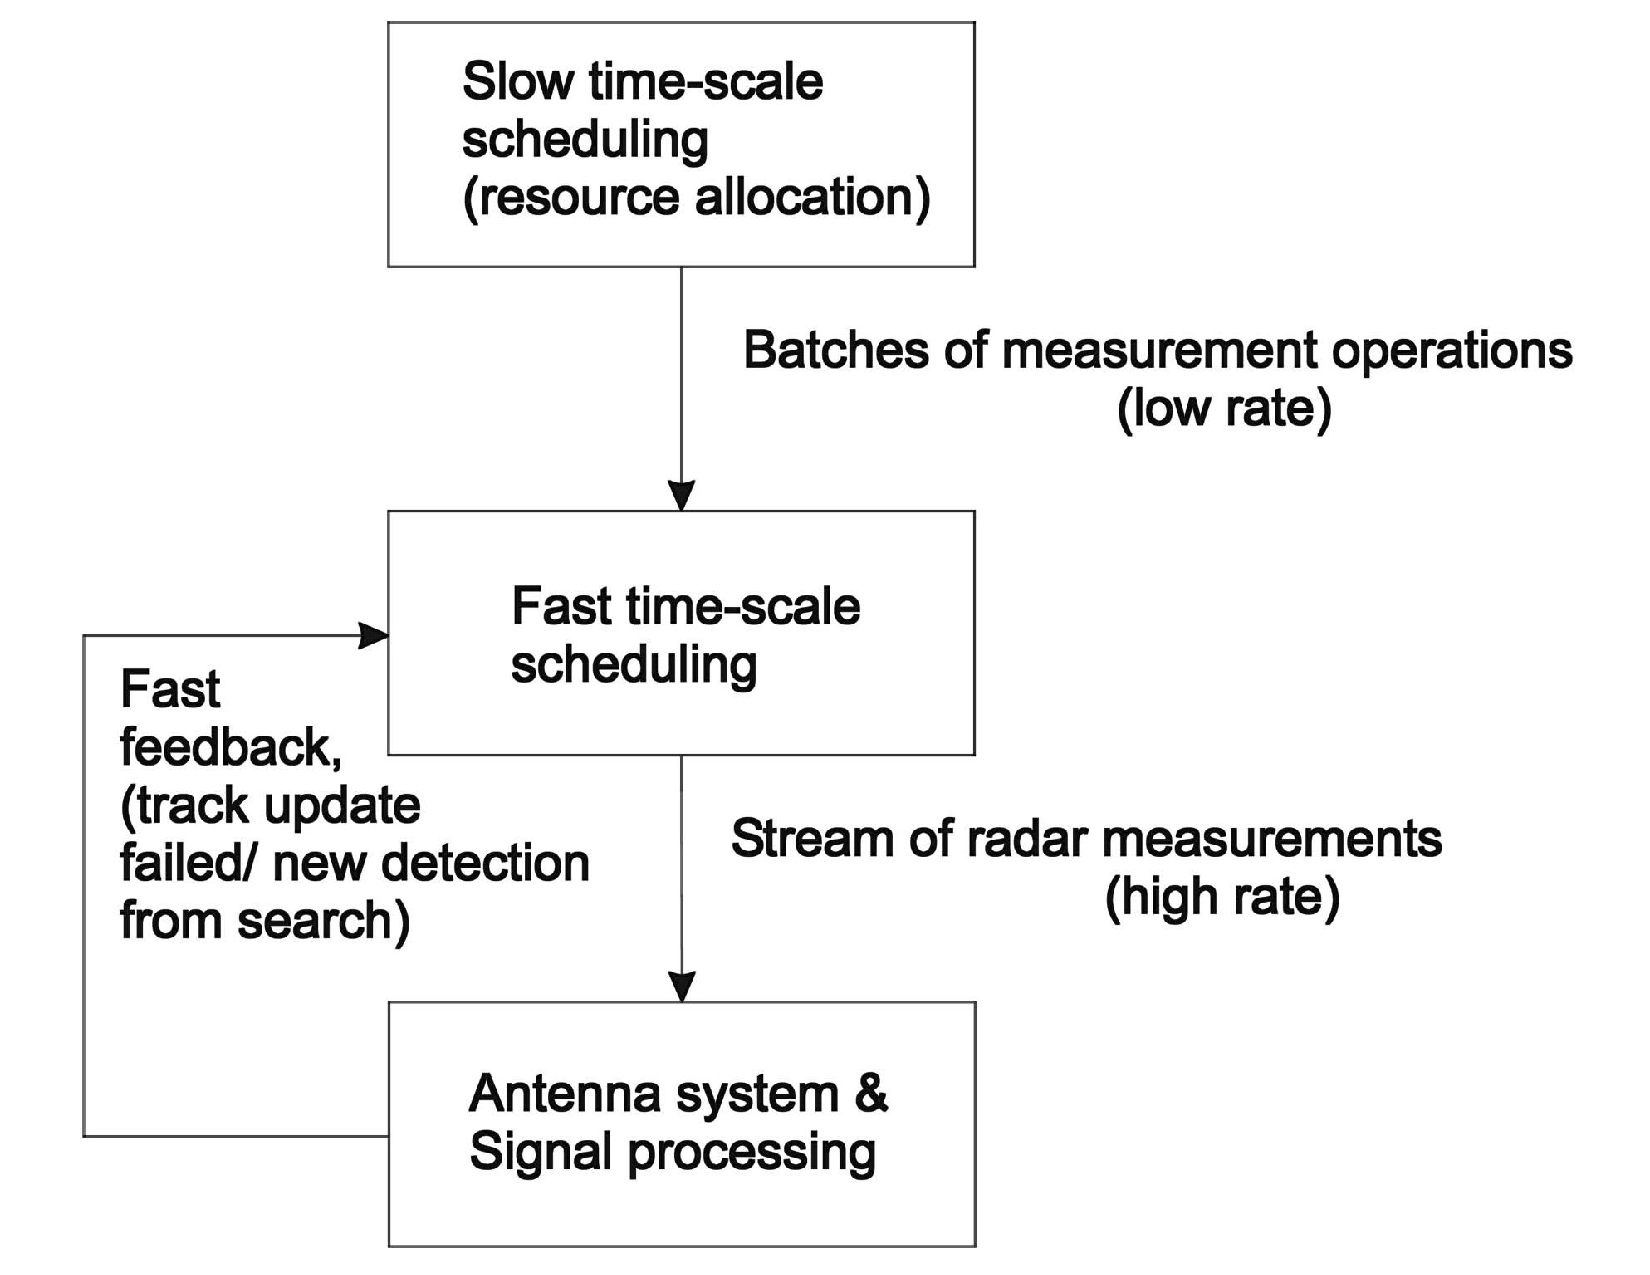
\includegraphics[width=0.5\textwidth]{figures/two_time_scale.pdf}
    \caption{Hierarchical resource management. Reprinted from \cite{Wintenby2006}.}
    \label{fig:tts_schdeuling}
\end{figure}

Winterby \etal proposed a convenient framework for solving the TBM problem as a constrained Markov decision process \cite{Wintenby2006}.
They acknowledged the fact that solving the TBM problem with conventional POMDP methodology is computationally intractable.
Therefore, the TBM problem was decomposed into slow-time-scale (STS) and fast-time-scale (FTS) scheduling objectives as shown in Figure \ref{fig:tts_schdeuling}.
The STS scheduler decides a batch of sensing tasks to be executed in the next time horizon.
The order of the tasks inside the batch is arranged by the FTS scheduler.
Moreover, it is assumed that the order of the tasks executed during the STS intervals is nonessential.
In \cite{Wintenby2006}, a sensing task is considered to be realized as an algorithm that generates sequence of sensing actions to achieve the goal of the task.
In target tracking, such algorithms can have for example repeated attempts to find a target in case of missing detections \cite{Wintenby2006}.
As a result, the sensing task execution times can be stochastic.
The STS scheduling problem was solved by formulating the Markov decision process as an optimization problem by using multiple different relaxations.
Even though multiple relaxation was made, the algorithm complexity is still too high for real-time implementation.


\subsubsection{Optimized dwell times for target tracking and search}

Byrne proposed in \cite{Byrne2015, Byrne2016} an optimization approach for scheduling radar dwells to minimize a cost function. 
The cost function was designed to handle search and tracking functions separately.
The dwell times for each radar task was optimized for the incoming scheduling interval, and constraints were applied to limit the sum of the dwell times below the duration of a scheduling interval.
First, a myopic cost function was optimized in \cite{Byrne2015}, and afterwards in \cite{Byrne2016} an approximate non-myopic approach was proposed to optimize the long-term costs.
The cost function was based on penalizing sensing actions that did not achieve track update or did not detect an undetected target.
Thus, costs for not detecting an undetected target in a surveillance area and not updating an existing track needed to be defined.
In addition, the cost function required defining a probability distributions for arriving targets, and cell transition probabilities for undetected targets.
The search space was discretized as in \cite{Kreucher2004} to simplify the computations.
The number of arriving targets to each grid cell was modeled with an independent Poisson distribution.
The transition probabilities for undetected targets were defined with a state transition kernel which describes the probability of a target moving from cell to another cell during the scheduling interval.
The overall cost function is formed by weighting the search and tracking costs by the probability that such event happens and summing all the weighted costs together.
The cost function emphasizes taking sensing actions that balance the overall search and tracking costs well based on the assumed probability distributions.

\subsection{Adaptive revisit interval algorithms for time budget management} \label{sec:tbm_ri}

The radar time resources can be released from tracking tasks by decreasing the revisit interval. 
The interval should be adjusted such that the track can be maintained and the tracking load is minimized.
Shorter revisit intervals should be used for maneuvering targets with higher process noise in order to maintain the quality of state estimates on a tolerable level. 
Similarly, longer revisit interval should be used for non-maneuvering targets with stationary trajectories because the movement is more predictable.
Different adaptive revisit interval algorithms have been widely studied to release time resources from target tracking to other radar tasks \cite{Cohen1986, Gardner1988, Munu1992, ChengTing2007, Baek2010, Watson1993, Charlish2015, Keuk1975, Shin1995, Benoudnine2006, Esfahani2012, Mofrad2017, Christiansen2018, Pilte2018}.
The algorithms are briefly covered in the following sections. 

\subsubsection{Residual based algorithms}

In \cite{Cohen1986}, Cohen \etal introduced a novel approach to adjust the revisit interval adaptively based on the innovation sequence of the tracking filter.
The innovation is the residual between the measurement $z(k)$ and the prediction $\hat{x}(k)$, and it is calculated as follows
\begin{equation}\label{eq:innovation}
    e(k) = z(k) - \hat{x}(k).
\end{equation}
The revisit interval was increased or decreased by using a simple recursive rule 
\begin{equation}\label{eq:update_resid}
    T(k) = \frac{T(k-1)}{\sqrt{e_n(k)}}.
\end{equation}
The signal $e_n(k)$ was calculated form $e(k)$ as follows
\begin{equation}\label{eq:norm_residual}
    e_n(k) = \frac{|e(k)|}{\sigma_m},
\end{equation}
which is absolute value of the innovation normalized with standard deviation of the measurement noise $\sigma_m$.
The equation \eqref{eq:innovation} was derived from the assumption that prediction error is proportional to the acceleration and to the square of the revisit interval.
For maintaining constant tracking error for maneuvering targets, the new revisit interval is inverse proportional to the last revisit interval and to the square root of the acceleration.
Consequently, the acceleration is unknown but the increase in acceleration is realized as increased errors in innovations.

In the simulations, an $\alpha \beta$ filter was used to track the target in two dimensions and the revisit interval was controlled using the equations \eqref{eq:innovation},\eqref{eq:norm_residual} and \eqref{eq:update_resid}.
A target trajectory with constant velocity and $90^\circ$ turn in a middle was used to evaluate the adaptive update interval algorithm.
The trajectory was noiseless such that the only noise present in the position measurements was induced by the measurement noise. 

In \cite{Gardner1988} the work in \cite{Cohen1986} was extended for $\alpha\beta\gamma$ filters in which the cube root of the normalized residual \eqref{eq:norm_residual} was used in the equation \eqref{eq:update_resid}.
Moreover, it was suggested that large variations in $e(n)$ can be smoothed by using a first-order low-pass filter.
The performance between the $\alpha\beta$ and the $\alpha\beta\gamma$ filters were compared in \cite{Munu1992}.
It was found out that $\alpha\beta\gamma$ filter can operate with longer update intervals than $\alpha\beta$ filter when the target is maneuvering.
Moreover, the cube root filter did achieve a better compromise between the tracking accuracy and the revisit interval.     
For constant velocity targets, the $\alpha\beta$ filter was more appropriate because it smooths the data better.

A residual-based algorithm for the IMM estimator was proposed in \cite{ChengTing2007}.
The following equation was obtained for calculating the revisit interval
\begin{equation}
    T(k) = \frac{4}{2^p}, \text{ } 4^p c < |e_s(k)| < 4^{p+1}c
\end{equation}
in which $e_s(n)$ is the normalized and smoothed residual.
Furthermore, equation for $p$ can be written as
\begin{equation}
    p = \floor*{\log_4\frac{1}{c}|e_s(k)|}
\end{equation}
where $c$ is variable that can be used to control trade-off between the accuracy and the tracking load.
Also, the maximum update interval was specified for the algorithm based on the used tracking models.

Baek \etal in \cite{Baek2010} proposed a residual-based algorithm in which the residual between the target position and the position estimate is wanted to keep below the desired threshold $e_\text{th}$.
A Kalman filter was used to track the target.
For the tracking filter, simple update rule was obtained
\begin{equation}\label{eq:update_baek}
    T(k) = T(k - 1) \sqrt{\frac{e_0}{|e(k)|}},
\end{equation}
where $e_0$ is the desired expected residual, which was derived from measurement error covariance matrix and desired threshold $e_\text{th}$ and target priority.
A higher target priority implies that lower revisit interval is used to reduce the probability of target moving out from the threshold area defined by $e_\text{th}$.
The equations \eqref{eq:update_resid} and \eqref{eq:update_baek} are effectively the same if $e_0$ is replaced with $\sigma_m$.


\subsubsection{Van Keuk's criterion}

Van Keuk proposed a criterion in \cite{Keuk1975} that can be utilized to calculate revisit interval efficiently for a target with known Signer model parameters.
Initially, the idea was considered in one-dimensional space.
The revisit interval optimization problem was formulated as a solution for the following criterion
\begin{equation} \label{eq:criterion}
    \sigma_p^2(k + T | k) = V_0^2 \sigma_m^2
\end{equation}
where $\sigma_p^2(k + T | k)$ is the position prediction error variance, $\sigma_m^2$ is the measurement error variance, and
the parameter $V_0$ was called track sharpness.
The approach assumed a Singer target model with acceleration standard deviation parameter $\Sigma$ and correlation parameter $\Theta$.
Using the assumed models and steady-state Kalman filter equations, a heuristic rule to calculate $T$ was obtained
\begin{equation}\label{eq:keuk_time}
    T \approx 0.4 \left[ \frac{\sigma_m \sqrt{\Theta}}{\Sigma} \right]^{0.4} \frac{V_0^{2.4}}{1+\frac{1}{2}V_0^2}
\end{equation}
which approximately fulfils the equation \eqref{eq:criterion}.
In higher dimensions, $\sigma_p^2(t + T | t)$ is the maximum eigenvalue of the predicted position error matrix, and $\sigma_m^2$ is the measurement error variance in the corresponding direction.

The equation \eqref{eq:keuk_time} was proposed in \cite{Keuk1975} for calculating the revisit interval efficiently but the optimal value for the track sharpness parameter $V_0$ was not considered.
However, the work was extended in \cite{vanKeuk1993} to find suitable value for $V_0$ by considering the tracking load
\begin{equation}\label{eq:load}
    L = \frac{\E{n}}{T}
\end{equation}
where $n$ is the number of dwells needed to obtain the detection.
It was assumed that only angular uncertainty needs to be considered when \eqref{eq:load} is minimized, 
because low uncertainty in the angle enables pointing the beam in the correct direction.
Therefore, the criterion \eqref{eq:criterion} was modified by replacing the parameter $\sigma_m^2$ with the half-power beamwidth $B$ of the transmitted beam, and the operations were done in U/V-coordinate system such that
\begin{equation} \label{eq:criterion2}
    G(t + T | t) = V_0 B
\end{equation}
where $G$ is the square root of predicted error standard deviation along the angular coordinate $u$. 
A refined version of the revisit interval rule was obtained based on the half-power beam width
\begin{equation}\label{eq:van_keuk_revisited}
    T \approx 0.4 \left[ \frac{\sigma_m r \sqrt{\Theta}}{\Sigma} \right]^{0.4} \frac{U^{2.4}}{1+\frac{1}{2}U^2}
\end{equation}
where $r$ is the distance from the radar to the target, and variance reduction parameter was defined as
\begin{equation}
    U = \frac{V_0 B}{\sigma_m}.
\end{equation}
The value for $V_0$ can be found by minimizing equation \eqref{eq:load} where $\E{n}$ and $T$ are substituted with their closed-form equations.

The research in \cite{Keuk1975, vanKeuk1993} was based on finding the formula to calculate the revisit interval for the Singer model with known maneuver parameters.
However, in \cite{Shin1995} the work was extended for IMM estimators where the maneuver parameters can be estimated online.
In other words, the maneuver parameters $\Theta$ and $\Sigma$ was calculated from the used IMM estimator models and their posterior model probabilities.
All the other results from Keuk's work could be still utilized as before.
Another Keuk's criterion based approach for IMM filters was proposed in \cite{Daeipour1994} where finite set of revisit intervals were defined.
The algorithm is straightforward, the closest interval that fulfill the equation \eqref{eq:criterion2} was searched exhaustively by using the prediction equations of the IMM estimator.


\subsubsection{Predicted error covariance based methods} \label{sec:error_covariance_methods}

The algorithms based on predicted error covariance matrix can be considered as a generalization of the Van Keuk's criterion.  
Novel work for optimizing the revisit interval to maintain desired state prediction error was carried out in \cite{Watson1993}.
The work was done for the IMM estimators for which the predicted error covariance matrix can be calculated by weighting the covariance matrices of the individual models with the model probabilities.
A threshold for the uncertainty was used which was proportional to the measurement error covariance matrix.
Furthermore, the threshold matrix and predicted covariance was set equal as follows  
\begin{equation}\label{eq:cov_th}
    \tr{ \vec{P}_{t+T|t} } = \tr{ \vec{P}_{\text{th}} }
\end{equation}
where $\vec{P}_{t+T|t}$ is the predicted error covariance, and $\vec{P}_{\text{th}}$ is the threshold covariance matrix.
From the equation \eqref{eq:cov_th}, a polynomial function was obtained which is a function of the revisit interval $T$.
The non-linear optimization problem was solved using Newton's method.



In \cite{Charlish2015} it is shown that it may be beneficial to introduce anticipation in the revisit interval algorithms.
The anticipation is utilized to prevent large prediction errors when the target moves through an occluded area.
This can be achieved by acquiring high prediction accuracy by using low revisit interval before the target moves to the occluded area where measurement accuracy is significantly reduced.
In other words, the POMDP framework was utilized where an immediate reward was defined as
\begin{equation}
    R(b_t, T) = \frac{u\left(\vec{P}_{t+T|t} \right) T}{\tau_c}
\end{equation}
where $b_t$ is the belief state, and $\tau_c$ is the measurement duration.
Moreover, the long-term rewards are calculated by using \eqref{eq:discounted_sum}.
The utility function $u\left(\vec{P}_{t+T|t} \right)=1$ if desired tracking accuracy is achieved.
Otherwise, a tracking accuracy below the threshold gradually decreases the utility function towards zero.



\subsubsection{Other approaches}

Benoudnine \etal proposed in \cite{Benoudnine2006} an IMM estimator with simplified architecture and a fast algorithm for calculating the revisit interval.
The IMM filter had two models, a constant velocity model, and a constant acceleration model.
The maximum revisit interval $\tmax$ was defined for the constant velocity model.
Similarly, the minimum revisit interval $\tmin$ was defined for the constant acceleration model.
The revisit interval was obtained with a simplified rule
\begin{equation}
    T = \muca \tmin + \mucv \tmax,
\end{equation}
where $\mucv$ and $\muca$ are the probabilities for constant velocity and constant acceleration models, respectively.

Masoumi-Ganjgah \etal proposed in \cite{Masoumi-Ganjgah2017} an algorithm which is closely related to algorithm proposed in \cite{Benoudnine2006}.
An IMM estimator with three different maneuver models was used, and parameters $\tmax$ and $\tmin$ was defined for the models.
The models was designed to have different maneuvering levels starting from low maneuvering model to high maneuvering model.
Also, the revisit interval was adjusted differently than in \cite{Benoudnine2006}.
The revisit interval was controlled recursively such that if the highest maneuvering model had the highest posterior probability, then 
revisit interval was decreased by multiplying it with a constant less than one.
On the other hand, if the lowest maneuvering model with had the highest posterior probability, then
revisit interval was increased by multiplying it with a constant scalar greater than one.
Otherwise, the revisit interval was kept the same as in the last interval.
The algorithm remind of residual based algorithms with a little bit different control policy.

Lastly, Esfahani and Kamarei in \cite{Esfahani2012} proposed a suboptimal non-myopic optimization method for solving the subset of tasks to be executed in the next scheduling interval.
However, the search task of the multifunction radar was not included in the formulation.
The approach was closely related to the adaptive update interval methods and hierarchical TBM methods.
It could be interpreted that the paper extends the adaptive update interval algorithms for multiple targets.
An algorithm was developed to find a subset of tracks to be updated in the next scheduling interval.
The objective was to maximize the target localization accuracy given the constraint on overall tracking load.
The non-myopic optimization problem was solved by utilizing the revisit intervals that minimize the individual tracing loads.
Moreover, the revisit intervals with the minimum loads were calculated by using the Van Keuk's results from \cite{vanKeuk1993}.
The approach approximates the non-myopic objective by calculating task deadlines by \eqref{eq:van_keuk_revisited}, and by scheduling tasks with closest deadlines for the current scheduling interval until the limit for the load is reached.

\newpage
\section{Reinforcement learning approach for revisit interval selection}

The optimal POMDP approach for TBM budget management was discussed to be intractable with conventional algorithms.
Reinforcement learning techniques could be used to find an approximate solution.
However, the observations and the actions are non-trivial to present for the reinforcement learning agent.
For example, in multitarget tracking the observation could be combination between belief states of each target, and the action could be to choose which tracks will be updated next.
The number of actions and the dimension of the observation are dependent on the number of targets.
Here the complexity of the observation and the action presentation problem can be avoided by utilizing some of the relaxations that were introduced in Chapter \ref{sec:literature_review}.
Especially, a reinforcement learning agent is trained to select suitable revisit interval in order to maximize the long-term reward function.  

The existing research on adaptive revisit interval algorithms was reviewed in Section \ref{sec:tbm_ri}.
It was identified that the existing algorithms control the revisit interval based on the innovation or the uncertainty on the estimates.
The residual based methods are less dependent on the target model since the average residuals are kept near the standard deviation of noise using a recursive rule \eqref{eq:update_resid}.
The covariance-matrix-based algorithms are less robust for model inaccuracies because the dynamic model is used to calculate the intervals.
However, the latter approach is more transparent since the prediction error covariance estimates are kept below a certain threshold.

The performance of an adaptive revisit interval algorithm is usually quantified by the achieved accuracy in the state estimates.
Especially, the position estimate is important for pointing the radar beam in the correct direction.
However, the purpose of applying adaptive revisit interval algorithms is to minimize the time allocated to tracking tasks.
The time allocation can be quantified with the track load which is the relation between the dwell time and the revisit interval \cite{vanKeuk1993}.

A commonly used tracking filter is an IMM estimator that can be used to track targets with various maneuvers as described in Section \ref{sec:IMM}.
The baseline IMM estimator consists of multiple Kalman filters which are configured for different maneuvers.
All the Kalman filters are concurrently used to track the targets.
The likelihood of an observation coming from a given Kalman filter state-space model can be extracted for each filter.
The probabilities can be used to calculate estimates for the process noise covariance matrix and the kinematic state.

Here a RL approach is proposed for controlling the revisit interval of the tracking task.
The RL agent is capable of learning directly from the experience such that 
system model is not needed to optimize the employed reward function.
Moreover, the approach should be modifiable to any tracking filter by defining suitable observation and reward space.
The motivation for using RL is to learn close to optimal policy which can adapt to any tracking system, allows learning a policy for learning non-myopic objectives as in \cite{Charlish2015}, and enables using observation data with non-trivial connection to the revisit interval.
The Section \ref{seq:system_description} starts by describing the employed radar system such that it is possible to identify the actions, observations and rewards for the RL formulation.
Thereafter, the RL formulation is described in Section \ref{sec:RL_formulation} 


\subsection{The system description} \label{seq:system_description}

\textcolor{red}{Content of this section is still in progress. It needs to be decided how much information is essential to put here. In addition, should the system be \textbf{exactly} like SAABs system or can it be modified etc. (general solution vs custom solution). What is essential information considering this thesis?}

The proposed RL approach is designed for an air surveillance radar that is capable to operate multiple missions concurrently.
In other words, the radar is a multifunction radar with AESA capabilities.
The radar is operating in challenging warfare scenarios such that it needs to be capable of detecting small targets in strong clutter and high-velocity targets.
Moreover, resistance to electronic countermeasures should be considered. 
Those requirements are concerned in each subsystem of the radar. 
Furthermore, the requirements should not be dismissed when the revisit interval selection algorithm is proposed.

The target tracking algorithm is assumed to be as given which takes into account the aforementioned requirements. 
The considered tracker is a multiple hypothesis tracker (MHT) coupled with an IMM estimator. 
The IMM estimator can adapt to different target maneuvers. 
However, tracking multiple targets creates a problem on how to associate the observations and the tracks to each other. 
The MHT solves the data association problem by associating all observations and tracks together combined with track likelihoods \cite{Blackman2004}. 
A track hypothesis is removed until a certain stopping rule is met. 

As the requirements are known, it is possible to consider how to formulate the revisit interval selection as an RL problem. The problem is initially approached by relaxing some of the requirements. However, it should be considered that the initial approach is expandable to a more general solution. 


What are the operational requirements?

\begin{itemize}
    \item Multimission radar
    \item General detection and tracking of air targets
    \item Capability of detection and tracking of small targets in strong clutter
    \item Capability of detecting and tracking of high velocity targets
    \item Capability of target detection during various forms of ECM, such as noise, DRFM and cover pulse
\end{itemize}

What are the actions that the agent can take?

\begin{itemize}
    \item Search( specified search volume, allowed time duration for the assigned task, required max. revisit time )
    \item Update Track (specified tracks, allowed time duration for the assigned task, required max revisit time per target)
\end{itemize}



\subsubsection{Tracker}

The particular tracking filter choice defines the available observations for the RL agent.
For example, the IMM estimator can provide model likelihoods, covariance estimates and innovation sequence that describe the current behaviour of the tracking system.
The tracker is implemented as an IMM estimator based on Kalman filters due to its simplicity and the popularity in real-world tracking systems.

\begin{itemize}
    \item Estimated values for positions and speed of different targets (3D), together with the covariances for these variables
    \item The history of each track (wrt. positions and speed as functions of time)
    \item A smoothed history of each track
    \item The class of each target, as estimated by the tracker, together with the likelihood for every target type
    \item Momentary acceleration (e.g. sideway acceleration for a turning aircraft)
    \item Association hypotheses and outliers (i.e. for what track each detection belongs to and whether it's considered an outlier by the tracker)
    \item Likelihoods for different behaviour modes of the targets, i.e. whether it's currently moving with constant velocity, performing a smooth turn, undergoing acceleration or making a heavy maneuver
    \item RCS, both for the hull and the rotors if applicable
\end{itemize}

\subsection{Formulating the revisit interval selection as RL problem}\label{sec:RL_formulation}

The reinforcement learning formulation starts by identifying the actions, observations and rewards.
It is essential to examine the observations if they fulfill the Markov property of Equation \eqref{eq:markov_property}.
If the Markov property is violated, next it should be determined if the problem is POMDP, and if the observation can be presented in a convenient belief state presentation.
Moreover, the belief state presentation can be used to solve POMDP problem as a continuous state MDP as described in Section \ref{sec:POMDP}.
In terms of utilizing strengths of RL approach, the downside of POMDP problems is that the presentation of the belief state typically requires a system model which increases the demand for human effort instead of letting the agent to learn by itself.

The next step is to determine suitable reinforcement learning algorithm to solve the problem.
The following questions will affect to the choice of the algorithm
\begin{enumerate}
    \item Is action space or state space continuous or have large cardinality? \label{enum:question_spaces}
    \item Is the maximization of the rewards essential during the learning? \label{enum:on_off_policy}
    \item Is the required learning time critical for the problem at hand? \label{enum:question_learning_speed}
    \item What are the computational resources available during the training? \label{enum:question_resources}
\end{enumerate}
\textcolor{red}{This introductory part will be continued in the near future...}

\subsubsection{Actions} \label{sec:actions}

The agent is the computer controlling the radar sensing actions.
The workflow of the agent is described as follows,
\begin{enumerate}
    \item Predict target position at the current time instant denoted as $t$. \label{enum:action_predict}
    \item Illuminate target at the predicted position.
    \item If detection obtained, correct the target state estimate with the obtained measurement. If no detection obtained, either return to step \ref{enum:action_predict} if the number missed detections is below a certain threshold, or otherwise remove the tracking task.
    \item Select the revisit interval $t_r$. \label{enum:action_rl_agent}
    \item Return to step \ref{enum:action_predict} at time instant $t+t_r$.
\end{enumerate}
All the steps except step \ref{enum:action_rl_agent} are controlled by conventional algorithms such as tracking filters.
The RL algorithm is only targeted to control the revisit interval parameter which a smaller part of the whole workflow.
There are two different ways for the agent to control the revisit interval.
The revisit interval could be selected directly from a set of intervals.
This approach will be referred as direct selections.
Another approach could either decrease or increase the revisit interval with certain delta values.
This approach will be referred as delta selections.
Both of the approaches could have a continuous or a discrete action space.
However, here only the discrete action spaces are considered.

The action space for the direct selection could be a set of revisit intervals where subsequent intervals have uniform distance.
In addition, the maximum revisit interval $\tmax$ and the minimum revisit interval $\tmin$ should be defined.
The parameters $\tmax$ and $\tmin$ can be derived from the employed dynamic models of the IMM estimator as in \cite{Benoudnine2006}.
An example of an arbitrary action space is $\{0.5, 1.0, 1.5, 2.0, 2.5\}$, where $\tmax=2.5$, $\tmin=0.5$ and size of the action space is $5$.
In general form, the action space is defined as follows
\begin{equation}\label{eq:as_direct}
    \As_\text{D} \coloneqq \{ \frac{n \tmax + (N-n-1) \tmin}{N-1} \}_{n=0}^{N-1},    
\end{equation}
where $N$ is the size of the action space.
The parameter $N$ could be interpreted as a hyperparameter.
Lower $N$ enables faster learning since there are less actions to be explored.
However, larger $N$ may enable higher performance since larger variety of revisit intervals could be used.

The delta selections could be defined such that equal number of decreasing or increasing delta values are defined.
Moreover, the deltas could be spaced uniformly as in \eqref{eq:as_direct}.
The maximum increase or decrease delta value is defined as a parameter $\deltalim$, which should be chosen along with the parameter $N$ to achieve sufficiently large deltas with satisfactory resolution.
An arbitrary action space for delta selections could be for example $\{ -1.0, -0.5, 0, 0.5, 1.0 \}$, where $\deltalim=1$ and $N=5$.
The general form for the action space can be defined as follows
\begin{equation}\label{eq:as_delta}
    \As_\Delta \coloneqq \{ \frac{\deltalim \left( 2 n - N + 1 \right)}{N-1} \}_{n=0}^{N-1},
\end{equation}
where $N$ should be positive odd number.
In opposite to the direct selections, defining $\tmax$ and $\tmin$ is not required, which enables the agent to learn suitable limits for revisit interval values.
However, the parameter $\tmin$ can be dependent on the radar parameters. 
For example, $\tmin$ should be larger or equal than the dwell time $\tau_d$.
Compared to the direct selections, a reaction speed to varying revisit interval requirements can be slower.
The reaction speed is dependent on how $\deltalim$ and $N$ are defined.
To address the aforementioned problem, it could be beneficial to define the delta values using a non-linear scale instead of the linear scale.

\subsubsection{Reward} \label{sec:rewards}

\begin{figure}[h]
    \centering
    \begin{subfigure}[b]{0.45\textwidth}
        \centering
        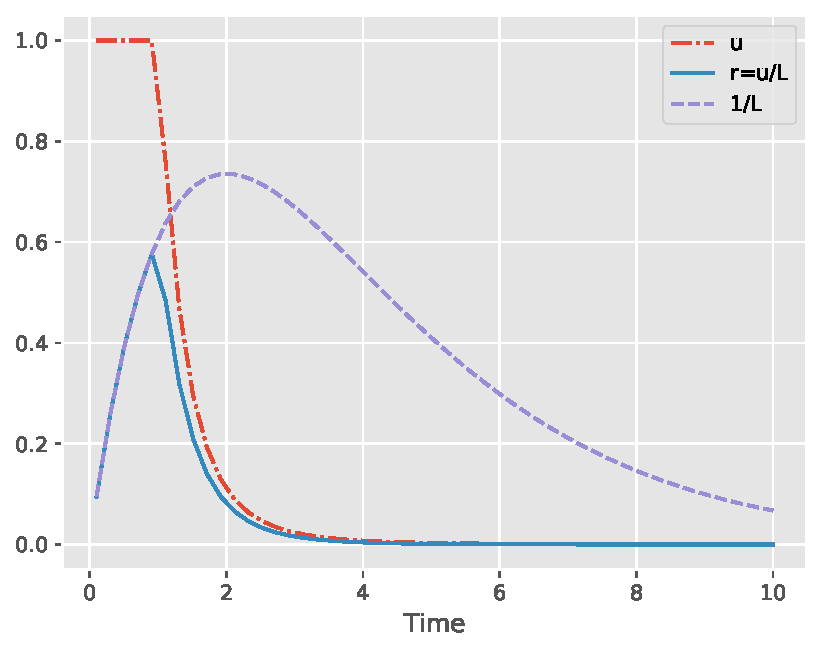
\includegraphics[width=\textwidth]{figures/reward.pdf}
        \caption{QoS term activates before minimum load is achieved.}
    \end{subfigure}
    \begin{subfigure}[b]{0.45\textwidth}
        \centering
        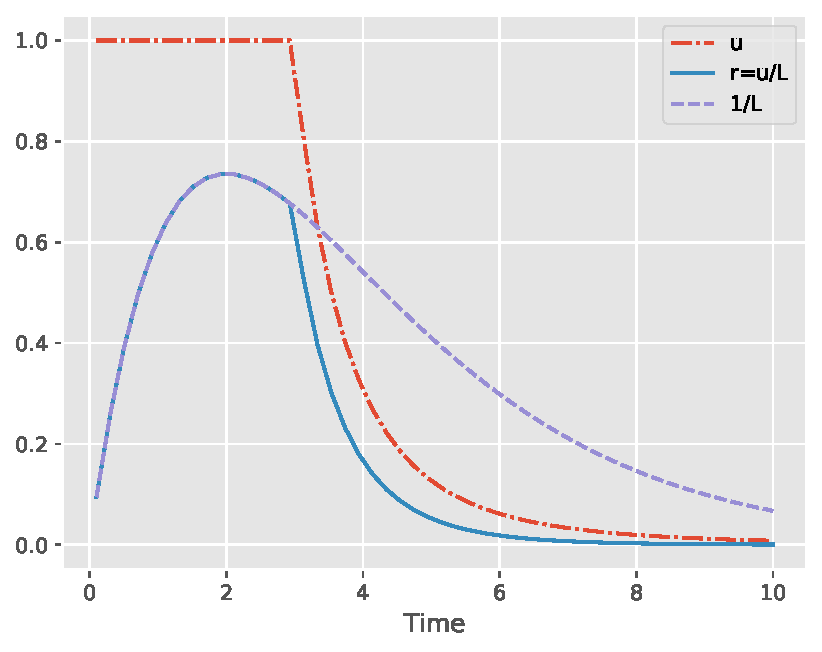
\includegraphics[width=\textwidth]{figures/reward2.pdf}
        \caption{QoS term activates after minimum load is achieved.}
    \end{subfigure}
    \caption{An example of a expected rewards at two different scenarios, where the Quality of Service (QoS) penalty is activated with different revisit intervals. \textcolor{red}{This is still temporary figure and will be updated in the near future.}
    }
    \label{fig:my_label}
\end{figure}

The reward function is used to give feedback for the agent on its actions.
In optimization, MDP and POMDP problems the objective is created using the system models.
However, in RL problems the rewards are based on events whose appearance is dependent on the action, the state and the previous state. 
An arbitrary example would be that, an optimization approach maximizes probability of detection but RL approach maximizes number of detections in a long run.
Obviously, rewards related to the probability of detection could be used in the RL approach but then the agent's ability to learn act optimally by its own is not fully utilized.
Moreover in cases where myopic policy is optimal, system model and rewards are fully known, conventional optimization algorithms are more efficient in finding the optimal action.

The radar is operating as a part of a larger system where the radar provides a snapshot of target position and radial velocity.
Since the observations does not contain the complete state information, the belief state is used.
The belief state is described by probability distributions that define the known information about the state variables.
In Section \ref{sec:Tracking}, the state variables of a target was modeled as Gaussian random variables which can be described by mean and covariance.
Other systems, utilizing the belief state given by the radar, can set Quality of Service (QoS) requirements on the certainty of the random variables.
Typically, the quality of the predictive error covariance matrix needs to be maintained above certain threshold as it was discussed in Section \ref{sec:error_covariance_methods}.

In some cases, the requirements set by other systems can be loose such that the radar needs to take into account the probability of losing or mixing tracks.
The costs for track losses and mixes can be defined depending on the attributes such as class and distance.
In the assumed radar system, the track is considered lost after $\nmax$ subsequent missed detections have occurred.
Therefore, the event of losing track is observable and can be included into reward function.
However, it can not be observed if any of the tracks are mixed.
Therefore, the probability of mixing tracks along with the mixing cost should utilized in the reward function.

\newcommand{\uqos}{u_\text{QoS}}
\newcommand{\closs}{c_\text{loss}}
The overall objective for the agent is to 
\begin{enumerate}
    \item minimize time budget needed to maintain the track, \label{enum:reward_tbm}
    \item keep the predicted estimates in a tolerable uncertainty level, \label{enum:reward_QoS}
    \item prevent track losses based on a cost of a track loss, and \label{enum:reward_losses}
    \item keep probability of mixing tracks below certain value. \label{enum:reward_mixes}
\end{enumerate}
From now on, the objectives \ref{enum:reward_QoS} and \ref{enum:reward_mixes} are combined such that only a single QoS objective is needed.
Therefore, the reward function is defined as follows
\begin{equation} \label{eq:reward}
    r(b, a) =
    \left\{
    \begin{array}{ll}
        \frac{t_r}{\tmax n} \uqos(b, a), & \text{in case of detection,} \\
        -\closs, & \text{otherwise.}
    \end{array}\right. 
\end{equation}
where $\tmax$ is used to normalize the rewards below $1$, $n \in \{1, 2, ..., \nmax\}$ is the number of dwells needed to achieve detection, $\closs$ is a penalty for a lost track, and $\uqos$ is a QoS penalty function.
The QoS penalty function is $1$ when the QoS objective is not violated and otherwise it gradually decreases towards zero.
Here $\uqos(b, a)$ is defined as follows
\begin{align}
    \uqos(b, a)
    &= \frac{\int_{t_0}^{t_0+t_r} \tr{\priorecovth} dt}{\int_{t_0}^{t_0+t_r}  g(\bm{\Sigma}_t) dt} \\
    &\approx \frac{\tr{\priorecovth} t_r}{\sum_{n=1}^{N} g(\bm{\Sigma}_{t+n\Delta_t}) \Delta_t} \label{eq:penalty_approximation}
\end{align}
where $N=\frac{t_r}{\Delta_t}$, $\Delta_t$ is an arbitrary processing sampling rate, $\priorecovth$ is a error covariance matrix given by the QoS requirement, and the function $g(\bm{\Sigma}_t)$ is defined as follows
\begin{equation}
    g(\bm{\Sigma}_t) =
    \left\{
    \begin{array}{ll}
        \tr{\bm{\Sigma}_t}, & \text{if } \tr{\bm{\Sigma}_t} < \tr{\priorecovth} \\
        1, & \text{otherwise.}
    \end{array}
    \right.
\end{equation}
The equation \eqref{eq:penalty_approximation} approximates the integral such that it is possible to calculate efficiently.

The reward function \eqref{eq:reward} defined similarly as in \cite{Charlish2015}.
However, $n$ is considered to be function of $t_r$ as in \cite{vanKeuk1993}, the possibility of a track loss is included, and $\uqos$ is defined differently.
The non-myopic objective \eqref{eq:discounted_sum} enables the RL approach to select actions which have non-maximum immediate rewards, but the long-term rewards are maximized.

\textcolor{red}{The reward function will be analyzed with more detail in the near future. Especially, the track loss cost needs to be explained better e.g. what happens in non-myopic case and relation to optimizing probability of track loss. Also, the reward can be formulated multiple different ways, this is the most reasonable I found out.}

\subsubsection{States and observations}

In Chapter $\ref{sec:MDP}$ it was briefly discussed what is the state in a Markov decision process.
The state describes the memoryless operation point of the system that is needed to know before taking an action.
In case of revisit interval selection, it is not trivial to define what is the actual state of the system.
One way to approach this problem is to identify an environment state and an agent state.
The environment state describes all the information that is needed to determine how the environment responds to actions of the agent.
On the other hand, the agent state contains the information that is relevant for the agent to choose an action.
Moreover, the achievable quality of the actions can be dependent on the amount of information is available.
In case where target states are described as hybrid systems, the environment state combines kinematic states for all targets and the states of the discrete stochastic processes.
The environment state is extracted by using a tracking filter such as IMM estimator.
The agent can affect to the sampling time instances but the actual target trajectories are assumed to be decoupled of the agent actions.

The agent can not observe the environment state directly, which is the reason for using the radar in the first place.
The agent state is related to the tracking filter and to the requirements set for the tracker.
In other words, the state is all the available information that is relevant for maximizing the reward function \eqref{eq:reward}.
The reward function was dependent on the tracking load, tracking losses, and QoS requirements.
The tracking load is dependent on how predictable the target state is.
If the tracking filter is optimal with correct model parameters, predictability of the target state is fully determined by the covariance matrix.
Therefore for a multiple model filter, $\modecovpost$, $\modexpost$ and $\mu_k^i$ for each more $i \in \{1, ..., M\}$ would be all the information needed to present the state.

In another case, where the filter is not optimal or the models are not accurate, innovation sequence is the only source to observe the real performance of the tracking filter.
The real performance of the tracking filter is reflected in the reward function as increasing tracking load and higher probability of tracking loss.
Therefore, innovation sequence should be utilized somehow to allow agent to prevent the increased tracking loss or the increased probability of losing track.
In particular, the expectation
\begin{equation} \label{eq:residual_expectation}
    \E{\xest - \z} = \xest - \E{\z} = \xest - \x
\end{equation}
could be interpreted as a state of the filter which is the residual between estimated state and the true state.
Unfortunately, the state is not fully observable and the tracking filter is already trying to minimize \eqref{eq:residual_expectation} in terms of MSE.
However, the innovation sequence can be used to detect if the tracking filter is approximately functioning as intended.
Especially, the innovation covariance is can be calculated by Equation \eqref{eq:kf_innov_cov}.
The same equation can be used to calculate the desired innovation covariance
\begin{equation}
    \innocov = \omodel \priorecovth \omodel + \ocov
\end{equation}
where $\priorecov$ is replaced by the error covariance from the QoS requirement $\priorecovth$.
The innovation covariance matrix can be decomposed by a eigenvalue decomposition into rotation component $\vec{U}$ and scaling component $\bm{\Omega}$.   
Thus, the measurement can be normalized to have unit covariance as follows 
\begin{equation}\label{eq:innov_norm}
    \tilde{\vec{y}}_n = \bm{\Omega}^{-\frac{1}{2}} \vec{U}\prefitinnov.
\end{equation}
In addition, the distance in the normalized space called Mahalanobis distance can be calculated as follows
\begin{equation}\label{eq:mahalanobis}
    D(\prefitinnov) = || \tilde{\vec{y}}_n ||_2 = \sqrt{\prefitinnov \innocov^{-1} \transpose{\prefitinnov}}
\end{equation}
Equations \eqref{eq:innov_norm} or \eqref{eq:mahalanobis} could be used as an observation.
In addition, as it was done in \cite{Gardner1988}, low-pass filtering may increase the performance. 

\textcolor{red}{This section is at the moment in progress. E.g. 
\begin{itemize}
    \item the correlations in the innovation sequence
    \item LSTM filters if they appear to be relevant at this point
    \item how the state presentation "looks like" for the agent
    \item is there any ways to simplify the state presentation (with all information presented here, the state presentation gets quite high dimension) e.g. using only the innovation sequence as they do in the residual based methods
\end{itemize}
}

\newpage
\section{Simulations}


In these simulations the reinforcement learning approach is trained in a simulated environment.
Essential metrics for comparing the reinforcement learning to other baseline algorithms are the tracking load and the prediction accuracy of the target position.
The categories for the baseline policies are the fixed revisit interval methods, the residual based algorithms, and the estimated prediction error covariance matrix based algorithms.
The simulation loop is implemented as follows
\begin{enumerate}
    \item Update target state.
    \item Predict target state using tracker.
    \item Query from the update policy if the track needs to be updated.
    \item If track update not needed return to step 1.
    \item Illuminate target at the predicted position with limited dwell length.
    \item If detection not obtained, end the simulation loop.
    \item Update the revisit policy and the tracker.
    \item Return to step 1.
\end{enumerate}
The loop is ran as long as the defined time horizon is reached in case when no track loss is experienced.
For simplicity, the algorithms are ran in two dimensional space instead in three dimensional space.

\subsection{Measurement model}

The simulated radar can measure the target position in polar coordinates such that radial $r$ and angular $\theta$ components are obtained.
Furthermore, the measurements are unbiased and distorted by uncorrelated Gaussian noise.
The noise covariance in Cartesian coordinates is approximated as follows,
\begin{equation} \label{eq:sim_ocov}
    \ocov = \rotmat 
    \left[
        \begin{array}{cc}
            \sigma_r^2 & 0 \\
            0 & r^2 \sigma_\theta^2
        \end{array}
    \right] 
    \transpose{\rotmat},
\end{equation}
where $\sigma_r^2$ is the noise variance of the radial component, $\sigma_\theta^2$ is the noise variance of the angular component, and $\rotmat$ is a two dimensional rotation matrix defined as
\begin{equation}
    \rotmat = \left[
        \begin{array}{cc}
            \cos(\theta) & -\sin(\theta) \\
            \sin(\theta) & \cos(\theta)
        \end{array}
    \right].
\end{equation}
The approximation of \eqref{eq:sim_ocov} is sufficiently accurate with low $\sigma_\theta$ values.
The noise variances $\sigma_\theta^2$ and $\sigma_r^2$ in polar coordinates are defined as
\begin{equation}
    \sigma_r^2 = c_r \SNR^{-\frac{1}{2}}
\end{equation}
and
\begin{equation}
    \sigma_\theta^2 = c_\theta \SNR^{-\frac{1}{2}}
\end{equation}
with appropriate constants $c_r$ and $c_\theta$.
Moreover, the SNR is assumed to be dependent on the angle predictions such that
\begin{equation}
    \SNR = \SN \cdot \exp{ - 2 \frac{\left(\theta - \hat{\theta} \right)^2}{B^2} },
\end{equation}
where $\hat{\theta}$ is the estimated target angle.
The center beam SNR $\SN$ is approximated to be constant because the radar can adaptively change the transmit power.
Lastly, the observation model is defined as follows
\begin{equation}
    \omodel = 
    \left[
        \begin{array}{cccccc}
            1 & 0 & 0 & 0 & 0 & 0 \\
            0 & 0 & 0 & 1 & 0 & 0
        \end{array}
    \right]
\end{equation}
since only the position components are measured.

\subsection{Target model}

Signer model is a state-space model in one dimensional space, where acceleration is modeled as Ornstein-Uhlenbeck process \cite{Pilte2018}.
The model can be extended for higher dimensions by using one model for each dimension.
The discrete time state transition matrix is defined as
\begin{equation}
\stmodel = 
    \left[
        \begin{array}{ccc}
            1 & T & \frac{\alpha T - 1 + \exp{-\alpha T}}{\alpha^2} \\
            0 & 1 & \frac{1 - \exp{- \alpha T}}{\alpha} \\
            0 & 0 & \exp{- \alpha T}
        \end{array}
    \right]
\end{equation}
where $\alpha$ is the correlation parameter of the acceleration noise.
Similarly, the process noise covariance matrix is written as
\begin{equation}
    \pcov = 2 \alpha \Sigma^2 
    \left[
    \begin{array}{ccc}
        \frac{T^5}{20} & \frac{T_4}{8}  & \frac{T^3}{6} \\
        \frac{T^4}{8}  & \frac{T^3}{3} & \frac{T^2}{2} \\
        \frac{T^3}{6}  & \frac{T^2}{2} & T
    \end{array}
    \right]
\end{equation}
where $\Sigma$ is the acceleration noise standard deviation.






\subsection{Results}

\begin{figure}
    \centering
    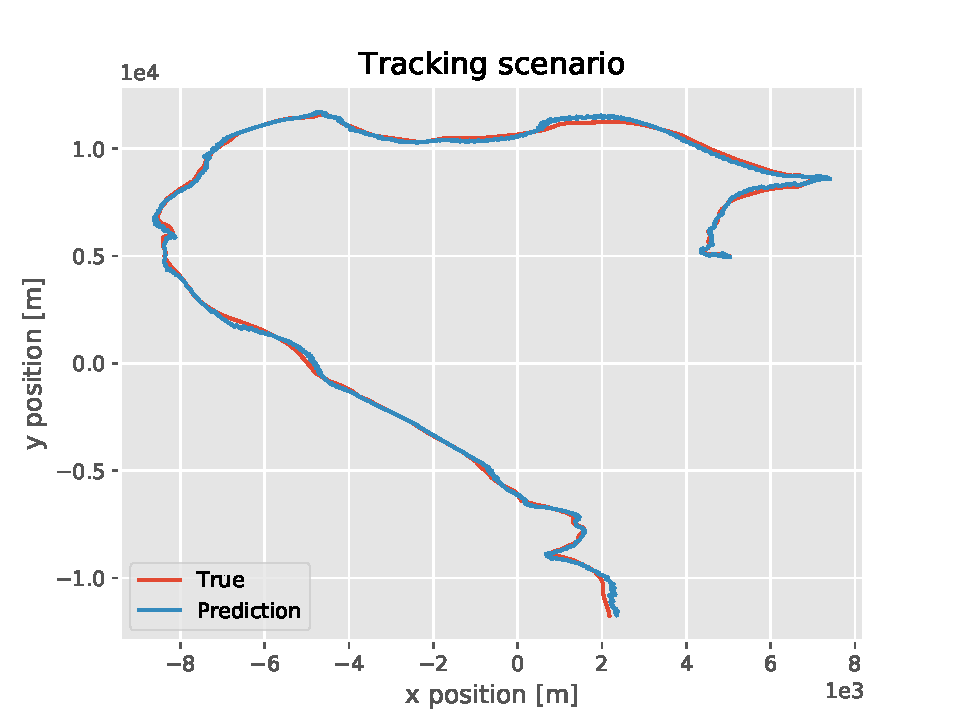
\includegraphics[width=\textwidth]{figures/simulations/scenario.pdf}
    \caption{Target trajectory and predicted target positions through the simulation.}
    \label{fig:sim_scenario}
\end{figure}

\begin{figure}
    \centering
    \begin{subfigure}[b]{0.45\textwidth}
        \centering
        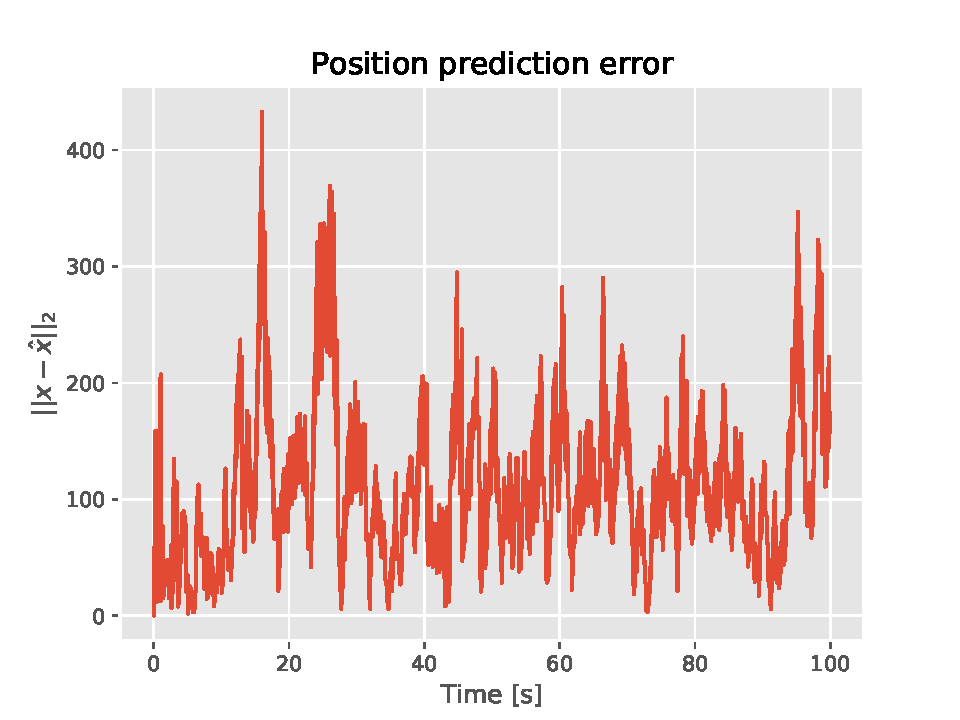
\includegraphics[width=\textwidth]{figures/simulations/position_error.pdf}
        \caption{Position error between target trajectory and position predictions.}
        \label{fig:sim_pos_error}
    \end{subfigure}
    \hfill
    \begin{subfigure}[b]{0.45\textwidth}
        \centering
        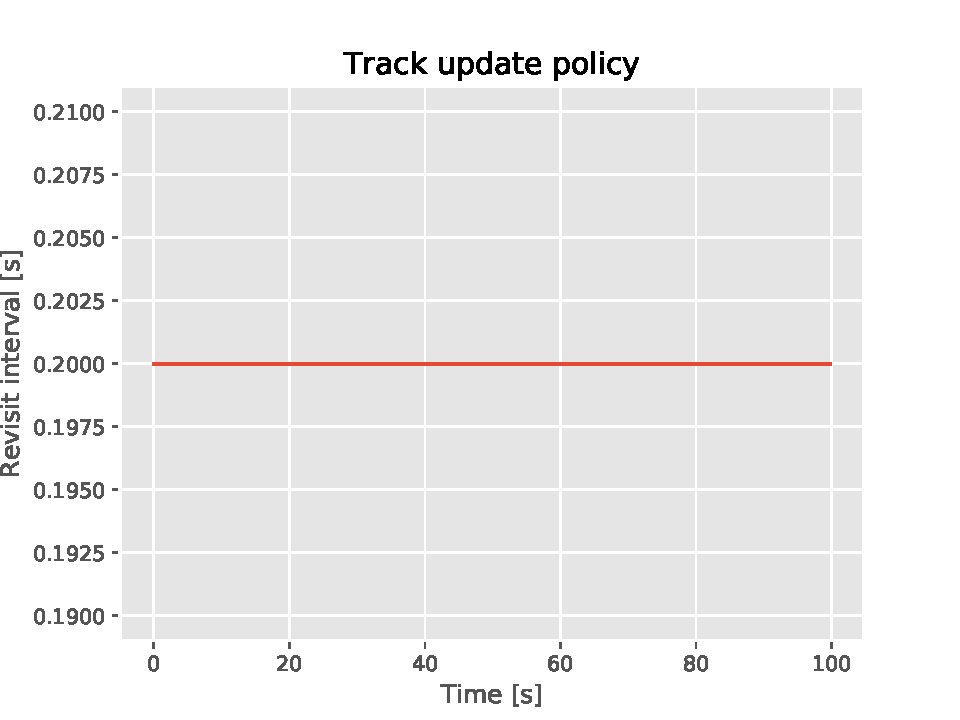
\includegraphics[width=\textwidth]{figures/simulations/update_policy.pdf}
        \caption{Update intervals used in the simulation.}
        \label{fig:sim_update_policy}
    \end{subfigure}
    \hfill
    \begin{subfigure}[b]{0.45\textwidth}
            \centering
            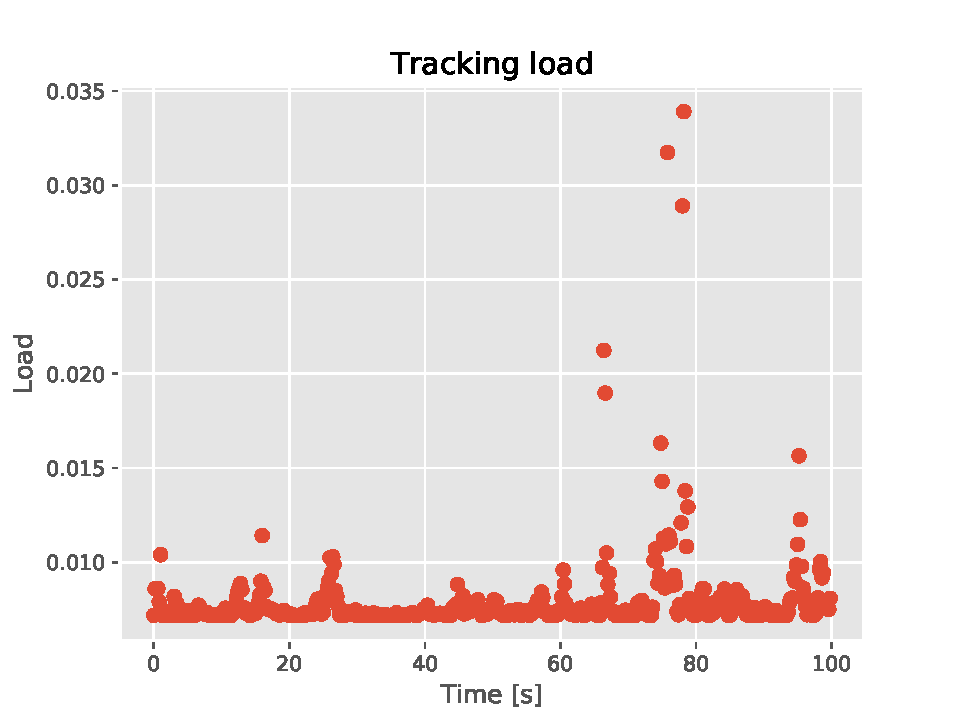
\includegraphics[width=\textwidth]{figures/simulations/load.pdf}
            \caption{Tracking load.}
            \label{fig:sim_load}
     \end{subfigure}
    \hfill
    \begin{subfigure}[b]{0.45\textwidth}
        \centering
        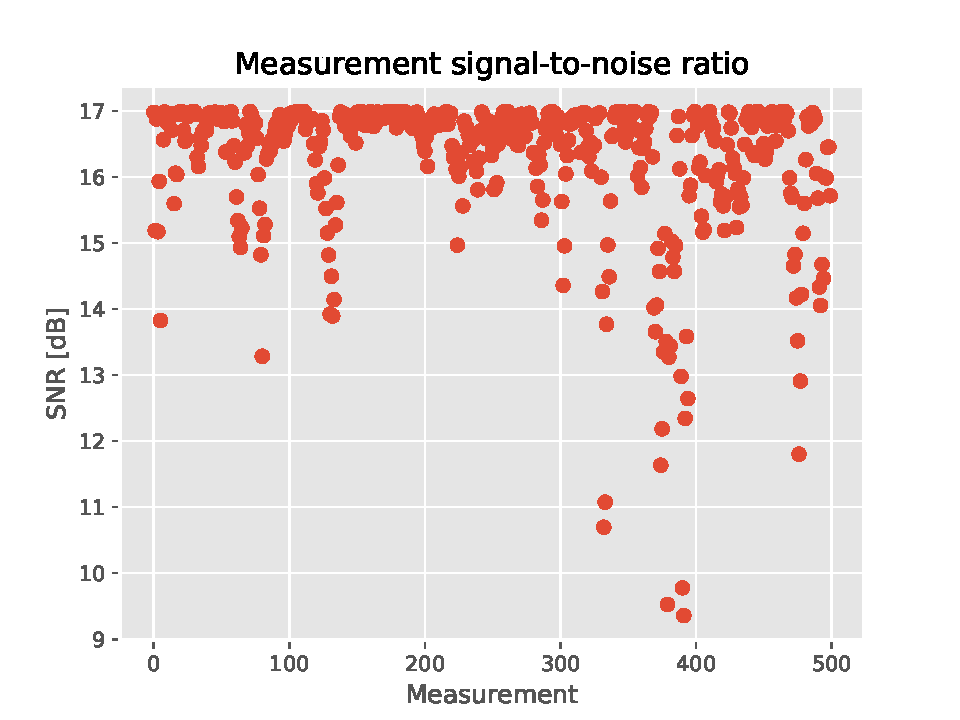
\includegraphics[width=\textwidth]{figures/simulations/snr.pdf}
        \caption{Measurement SNR.}
        \label{fig:sim_snr}
    \end{subfigure}
     
    \caption{Simulation metrics for constant update rate policy.}
    \label{fig:three graphs}
\end{figure}

\newpage
\section{Conclusions}


\thesisbibliography

\printbibliography


\end{document}
